%% This is file `elsarticle-template-1-num.tex',
%%
%% Copyright 2009 Elsevier Ltd
%%
%% This file is part of the 'Elsarticle Bundle'.
%% ---------------------------------------------
%%
%% It may be distributed under the conditions of the LaTeX Project Public
%% License, either version 1.2 of this license or (at your option) any
%% later version.  The latest version of this license is in
%%    http://www.latex-project.org/lppl.txt
%% and version 1.2 or later is part of all distributions of LaTeX
%% version 1999/12/01 or later.
%%
%% The list of all files belonging to the 'Elsarticle Bundle' is
%% given in the file `manifest.txt'.
%%
%% Template article for Elsevier's document class `elsarticle'
%% with numbered style bibliographic references
%%
%% $Id: elsarticle-template-1-num.tex 149 2009-10-08 05:01:15Z rishi $
%% $URL: http://lenova.river-valley.com/svn/elsbst/trunk/elsarticle-template-1-num.tex $
%%
\documentclass[preprint,12pt]{elsarticle}
\usepackage{amsmath}
\usepackage{graphicx,subcaption}
\usepackage{listings}
\usepackage{hyperref}
\usepackage{multirow}
\usepackage{notoccite}
\hypersetup{
    colorlinks,
    citecolor=black,
    filecolor=black,
    linkcolor=black,
    urlcolor=black
}

%% Use the option review to obtain double line spacing
%% \documentclass[preprint,review,12pt]{elsarticle}

%% Use the options 1p,twocolumn; 3p; 3p,twocolumn; 5p; or 5p,twocolumn
%% for a journal layout:
%% \documentclass[final,1p,times]{elsarticle}
%% \documentclass[final,1p,times,twocolumn]{elsarticle}
%% \documentclass[final,3p,times]{elsarticle}
%% \documentclass[final,3p,times,twocolumn]{elsarticle}
%% \documentclass[final,5p,times]{elsarticle}
%% \documentclass[final,5p,times,twocolumn]{elsarticle}

%% if you use PostScript figures in your article
%% use the graphics package for simple commands
%% \usepackage{graphics}
%% or use the graphicx package for more complicated commands
%% \usepackage{graphicx}
%% or use the epsfig package if you prefer to use the old commands
%% \usepackage{epsfig}

%% The amssymb package provides various useful mathematical symbols
\usepackage{amssymb}
%% The amsthm package provides extended theorem environments
%% \usepackage{amsthm}

%% The lineno packages adds line numbers. Start line numbering with
%% \begin{linenumbers}, end it with \end{linenumbers}. Or switch it on
%% for the whole article with \linenumbers after \end{frontmatter}.
\usepackage{lineno}

%% natbib.sty is loaded by default. However, natbib options can be
%% provided with \biboptions{...} command. Following options are
%% valid:

%%   round  -  round parentheses are used (default)
%%   square -  square brackets are used   [option]
%%   curly  -  curly braces are used      {option}
%%   angle  -  angle brackets are used    <option>
%%   semicolon  -  multiple citations separated by semi-colon
%%   colon  - same as semicolon, an earlier confusion
%%   comma  -  separated by comma
%%   numbers-  selects numerical citations
%%   super  -  numerical citations as superscripts
%%   sort   -  sorts multiple citations according to order in ref. list
%%   sort&compress   -  like sort, but also compresses numerical citations
%%   compress - compresses without sorting
%%
%% \biboptions{comma,round}

% \biboptions{}

\let\originaleqref\eqref
\renewcommand{\eqref}{Eq.~\originaleqref}

\hypersetup{colorlinks=true,
  pdftitle={Performance and Accuracy of Criticality Calculations Performed Using WARP, A Framework for Continuous Energy Monte Carlo Neutron Transport in General 3D Geometries on GPUs},
  pdfauthor={Ryan M. Bergmann, Kelly L. Rowland, Nikola Radnovi\'c, Rachel N. Slaybaugh, Jasmina L. Vuji\'c}}

\journal{Annals of Nuclear Energy}

\begin{document}

\begin{frontmatter}

%% Title, authors and addresses

%% use the tnoteref command within \title for footnotes;
%% use the tnotetext command for the associated footnote;
%% use the fnref command within \author or \address for footnotes;
%% use the fntext command for the associated footnote;
%% use the corref command within \author for corresponding author footnotes;
%% use the cortext command for the associated footnote;
%% use the ead command for the email address,
%% and the form \ead[url] for the home page:
%%
%% \title{Title\tnoteref{label1}}
%% \tnotetext[label1]{}
%% \author{Name\corref{cor1}\fnref{label2}}
%% \ead{email address}
%% \ead[url]{home page}
%% \fntext[label2]{}
%% \cortext[cor1]{}
%% \address{Address\fnref{label3}}
%% \fntext[label3]{}

\title{Performance and Accuracy of Criticality Calculations Performed Using WARP, A Framework for Continuous Energy Monte Carlo Neutron Transport in General 3D Geometries on GPUs}

%% use optional labels to link authors explicitly to addresses:
%% \author[label1,label2]{<author name>}
%% \address[label1]{<address>}
%% \address[label2]{<address>}

\author{Ryan M. Bergmann\corref{rmb}}
\ead{ryanmbergmann@gmail.com}
\cortext[rmb]{Corresponding author. Tel.: +41.76.687.53.09.}

\author{Kelly L. Rowland}
\ead{krowland@berkeley.edu}

\author{Nikola Radnovi\'c}
\ead{radnovicn@gmail.com}

\author{Rachel N. Slaybaugh}
\ead{slaybaugh@berkeley.edu}

\author{Jasmina L. Vuji\'c}
\ead{vujic@nuc.berkeley.edu}


\address{Department of Nuclear Engineering, 
4155 Etcheverry Hall, 
University of California - Berkeley,
Berkeley, CA 94720-1730}

\begin{abstract}

In this companion paper to ``Algorithmic Choices in WARP - A Framework for Continuous Energy Monte Carlo Neutron Transport in General 3D Geometries on GPUs'' (doi:10.1016/j.anucene.2014.10.039), the WARP Monte Carlo neutron transport framework for GPUs is benchmarked against production-level CPU Monte Carlo neutron transport codes for both performance and accuracy.  Flux spectra and multiplication factors calculated by WARP are compared to those from Serpent 2.1.21 and MCNP 6.1 for identical materials and geometries.  Runtimes, speedup factors, and cost comparisons are also reported.

\end{abstract}

\begin{keyword}
Monte Carlo \sep Neutron Transport \sep GPU \sep CUDA \sep CUDPP \sep OptiX


\end{keyword}

\end{frontmatter}

\linenumbers

%% main text

\section{Introduction}
\label{sec:intro}

%I would add an introductory paragraph here mentioning that warp solves the neutron transport equation, that the specific application is reactor physics, and the overall goals of the project. The current start is a bit out of nowhere.
% RMB - added intro from last paper
WARP, which can stand for ``Weaving All the Random Particles,'' is a three-dimensional (3D) continuous energy Monte Carlo neutron transport code developed at UC Berkeley to efficiently execute on a CPU/GPU platform.  WARP accelerates Monte Carlo simulations while preserving the benefits of using the Monte Carlo method, namely, that very few physical and geometrical simplifications are applied.  WARP is able to calculate multiplication factors, flux tallies, and fission source distributions for time-independent problems, and can run in both criticality or fixed source modes (but fixed source mode is not robust or optimized).  WARP can currently transport neutrons in unrestricted arrangements of parallelepipeds, hexagonal prisms, cylinders, and spheres.

The impetus for developing WARP was the research done by Martin and Brown in 1984 \cite{vector} for Monte Carlo and by Vuji\'{c} and Martin in 1991 \cite{vujic_vector} for collosion probability method.  In the 1984 paper, a method for mapping the Monte Carlo problem onto SIMD (single instruction multiple data) vector computers is described.  SIMD is an execution model some processors use in order to lower the number of instructions needed per amount of computation done, which increases both power and computational efficiency \cite{simd_power}.  SIMD requires the same instructions to be carried out over every element in a concurrently-processed data vector.  The essential idea in the 1984 paper is to bank the neutrons into vectors based on their required operation.  If a neutron is scattering, its data is placed in the scattering buffer.  If a neutron needs to do a surface crossing, it is put in the crossing buffer, and so on.  Once a buffer becomes full, it is processed in a SIMD fashion by the vector computer.  Processing the neutrons makes the buffers contain non-uniform reactions, however, and a ``shuffle'' operation is done that actually moves data back into contiguous blocks based on the reaction type.  

This new approach was named ``event-based'' Monte Carlo, since the neutron events are tracked and processed as a group \cite{vector}.  This was a very different way of performing a Monte Carlo simulation at the time.  Almost all computers were strictly serial, and SIMD lanes were only available in supercomputers.  Therefore, the pervasive method was the ``task-based" method in which neutrons are tracked for their entire lifetime in series.  Since GPUs are massively parallel and rely on SIMD, an event-based algorithm seems to be the appropriate approach to GPU-accelerated neutron transport.  

WARP uses an event-based algorithm, but with some important differences.  Vectorizing the Monte Carlo algorithm should allow for efficient GPU execution, but a paper by Zhang \cite{on_the_fly_remapping} also shows that by remapping data references, the thread divergence in GPU warps can be minimized.  Moving data is expensive, so WARP uses a remapping vector of pointer/index pairs to direct GPU threads to the data they need to access.  The remapping vector is sorted  by reaction type after every transport iteration using a high-efficiency parallel radix sort, which serves to keep the reaction types as contiguous as possible and removes completed histories from the transport cycle.  Sorting reduces the amount of divergence in GPU ``thread blocks,'' keeps the SIMD units as full as possible, and eliminates using memory bandwidth to check if a neutron in the batch has been terminated or not.  Using a remapping vector means the data access pattern is irregular, but this is mitigated by using large batch sizes where the GPU can effectively eliminate the high cost of irregular global memory access.

The goal of WARP is to be the first step in creating a full-featured, continuous energy, Monte Carlo neutron transport code that is \emph{accelerated} by running on GPUs.  The crux of the effort is to make Monte Carlo calculations faster while producing accurate results.  Modern supercomputers are commonly being built with graphics processing units (GPU) coprocessor cards in their nodes to increase their computational efficiency and performance.  Compared to more common central processing units, or CPUs, GPUs have a larger aggregate memory bandwidth, much larger rate of floating-point operations per second (FLOPS), and lower energy consumption per FLOP.  GPUs execute efficiently on data-parallel problems, and since most CPU codes are task-parallel, the algorithms used had to be reconsidered.  Data-parallelism is simply parallelism that arises from operating on many different pieces of data at one time, whereas task-parallelism is parallelism that arises from running many concurrent tasks that act on a single piece of data.   Figure \ref{datavtask} shows an illustration of the difference between a data-parallel and a task-parallel neutron transport loop.

\begin{figure}[h!] 
  \centering
    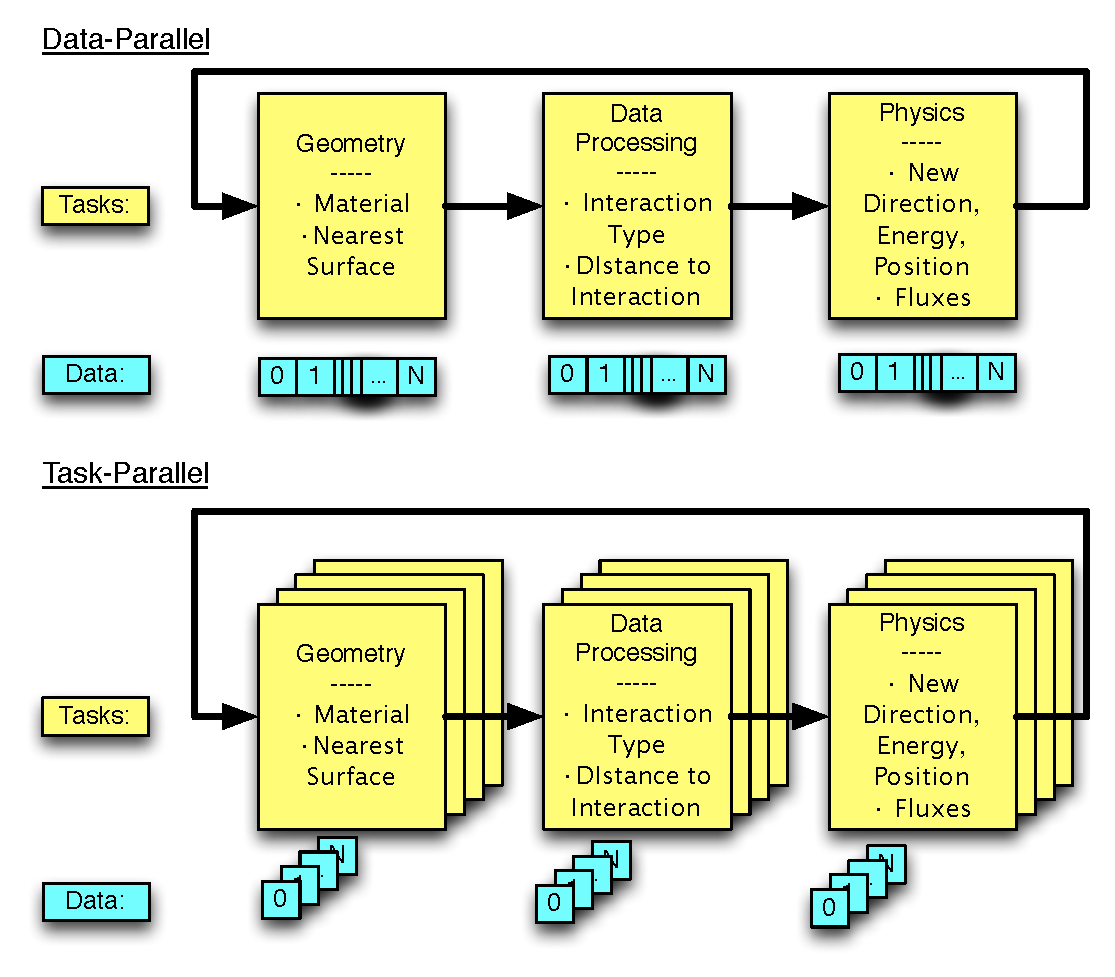
\includegraphics[width=\textwidth]{graphics/datavtask.pdf}
     \caption{Data-parallel neutron trasport loop vs.\ a task-parallel transport loop for transporting N neutrons in parallel.  \label{datavtask} }
\end{figure}

Execution on GPUs requires strategic data management since the on-chip memory of the GPU is separate from the host CPU's memory \cite{cuda}. To use NVIDIA GPUs, parts of software must be written in a language that facilitates interaction with the GPU. We chose CUDA \cite{cuda}, a set of extensions for C/C++.  
%You may want to add a sentence here about the need to use a different MC algorithm than the standard approach (you mention data parallel vs. task parallel, but you don't say how that relates to MC). This would provide some cohesion. %RMB - added more intro from last paper.  This also can't be my dissertation.  We have to assume that the audience as some familiarity.
The simplest way to accommodate all these requirements was to write a new code from scratch, which ultimately resulted in WARP.  

In this paper, the features of WARP are summarized while highlighting the newest developments, the results of criticality calculations performed by WARP are compared against those from Serpent 2.1.21 \cite{jaakko,serpent} and MCNP 6.1 \cite{mcnp6}, two widely-used production-level Monte Carlo neutron transport codes, in order to ensure the accuracy of WARP and to highlight its performance differences, and lastly a discussion is given summarizing the .  The details about the algorithms used in WARP are discussed in \cite{algorithms} and will not be discussed in detail here.
%Here I'd more fully outline the paper. It is common to give a section-by-section breakdown.


%%%%%%%%%%%%%%%%%%%
%%%%%%%%%%%%%%%%%%%
%%%%%%%%%%%%%%%%%%%
\section{Features of WARP}
\label{sec:features}

WARP has only existed since 2013, and is not as fully-featured as more mature Monte Carlo codes.  However, it has the functionality necessary to compare its performance against Serpent 2.1.21 and MCNP 6.1, and this section outlines the current set of features available in WARP.  

\subsection{Physics}

Only neutrons are transported by WARP.  Any other particles are not considered in any way.  WARP loads ACE-formatted nuclear data libraries via the ``ace'' module in PyNE (Python for Nuclear Engineering) \cite{pyne}.  This module has been separated and included as a standalone Python module with WARP.  Including it with WARP in this way means the entire PyNE package does not need to be installed in order to compile and run WARP (reducing the level of ``dependency hell'').  The cross section data are then re-formatted to use a unionionzed energy grid via NumPy \cite{numpy}, the re-formatted data are then passed to the C++ routines via the Python C API.  Cross section data compiled by the United States is distributed by the Department of Energy in \emph{ENDF} files.  ENDF stands for ``evaluated nuclear data file'' and can contain data for nuclear decay, photons, atomic relaxation, fission yields, thermal neutron scattering, and charged particle reactions as well as neutron reactions.  ACE stands for ``a compact ENDF'' and strips out much of the extra information unnecessary for neutron transport and formats the data into the specified tabulation \cite{endfnums}.  Since many Monte Carlo codes read ACE-formatted data rather than the original ENDF file, WARP can eliminate one potential cause for discrepancies by loading the same data as other codes.  

In its current state, WARP does not use S($\alpha,\beta$) thermal scattering tables or unresolved resonance parameters and only uses the free-gas approximation for target nuclei.  The free-gas approximation treats the target as part of a gas at a certain temperature and does not consider other modes of energy transfer that rise from inter- and intra-molecular phenomena.  Thermal scattering and unresolved resonance data improve the physical fidelity of the simulation, but these features can be turned off in production codes so that WARP can be directly compared to them.  The incorporation of S($\alpha,\beta$) thermal scattering tables or unresolved resonance parameters in WARP could lead to more divergent program flow and is therefore an area for future investigation.

WARP currently also has an incomplete set of the ENDF sampling laws implemented: laws 3 (level scattering), 4 (continuous tabular distribution), 7 (simple Maxwell fission spectrum), 9 (evaporation spectrum), 11 (energy-dependent Watt spectrum), 44 (Kalbach-87 formalism), 61 (LAW=44 but tabular angular distribution), and 66 (N-body phase space distribution) \cite{MCNP}.  These laws cover all the reactions present in the test problems presented here and most nuclides in the ENDFB/VII.1 cross section data set, but some nuclei may have interactions that require the remaining neutron sampling laws: 1 (tabular equiprobable energy bins), 5 (general evaporation spectrum), 22 (tabular linear functions), 24 (UK law 6), 67 (laboratory angle-energy law).  Problems containing any such nuclides cannot be simulated according to the data specifications with the current version of WARP, but of course could be added later.  These law are not nearly as common as the ones currently included in WARP, and excluding them at this point should not greatly reduce the ability to benchmark the performance and accuracy of WARP.
% You may want to mention whether any of the ones left out are important or state that they aren't important for the problems we care about or something along those lines. Brief information about whether this is important would be helpful.

Sophisticated variance reduction is also not implemented in WARP.   WARP does use neutron weight to calculate fluxes and multiplication factors, so simple variance reduction techniques like implicit capture should be a straight-forward part of future development. Currently, the only reactions that adjust neutron weight are multiplicity reactions, like (n,2n), where the neutron weight is multiplied by the exiting neutron number in a manner similar to OpenMC \cite{openmc}.  This means that new neutron histories do not have to be created mid-batch in criticality calculations, and makes program flow simpler.  

\subsection{Geometry}

The geometry representation in WARP is handled by the NVIDIA OptiX library [citation].  OptiX provides good performance on the GPU, but imposes some limitations on the how geometries must be input and that restricts the kinds of benchmarks that can be done. Pertinent limitations are:

\begin{enumerate}
\item Cells are the basic building blocks, not surfaces.
\item All cells must be finite, closed, and non-overlapping.
\item Implicit nesting determines what material exists inside of a cell.  In other words, since cells are defined directly, the material of cell A is only that space where cell A is the lowest nested cell.  If cell B is within cell A, the entire space within cell B is excluded from cell A simply because cell B resides within cell A and does not need to be excluded explicitly.
\item The only cell types available are spheres, cylinders, right rectangular prisms, and right hexagonal prisms.
\item Only translational transforms have been implemented, although this restriction could be lifted by some additional development.
\item Vacuum (i.e.\ infinitely absorbing) and specular reflection  (i.e.\ mirror) boundary conditions are available.  Periodic boundary conditions have not yet been implemented.
\end{enumerate}

An improved tracking routine has been implemented in WARP since the last publication \cite{algorithms}.  WARP now uses ``cell sense'' to reduce the memory impact of determining in which cell/material a neutron resides.  ``Cell sense'' is like surface sense in that it is positive if a neutron is outside a cell and is negative if a neutron is inside the cell. Cell sense is simply the product of the surface senses of the cell's constituent planes.  In other words, the surface normals in WARP always point outward, and the signs of the normals encountered are summed along a trace.  When the sum becomes negative, the last intersected surface is the cell in which the neutron is located.  Figure \ref{whereami} shows an illustration of this process.

\begin{figure}[h!]
\centering
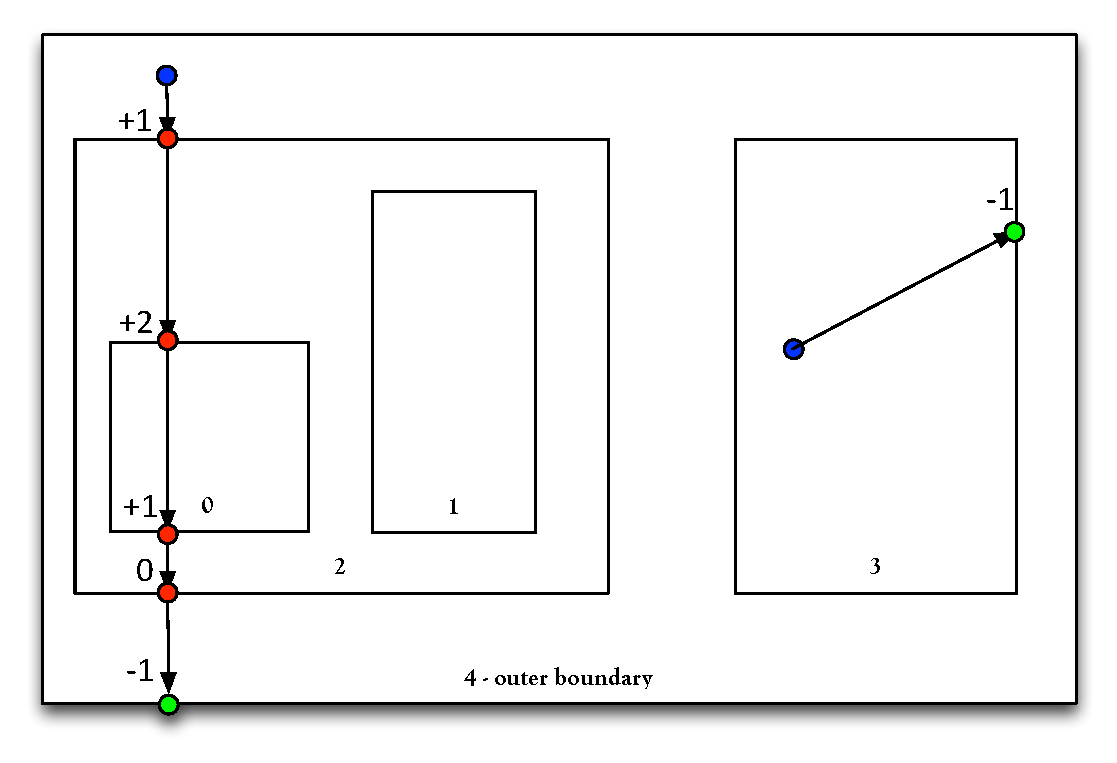
\includegraphics[width=0.75\textwidth]{graphics/whereami-new.pdf}
\caption{The improved point-in-polygon ``where am I?'' algorithm. \label{whereami} }
\end{figure}

Previously, a list of cell numbers was stored for each intersection and the double entries removed to give a nesting list for the neutron.  Now, the cell sense (which is either 1 or -1) is calculated and summed as the query ray traverses the geometry.  When the cumulative sense becomes negative, the containing cell has been intersected and tracing can stop.  This can be done because all bodies must be closed.  This scheme takes advantage of the acceleration structure in OptiX while still using the simplicity of combinatorial solid geometry.  It essentially is the same scheme as MCNP/Serpent, except that the acceleration structures allow surfaces that are part of cells that are far away to be skipped.  Also, compared to the past scheme of storing a list of doubles, this method requires a single integer to be stored and operated on instead of a (potentially large and slow) list. This change should reduce the memory required by the geometry tracking routine.
% or some final sentence like that. It is not explicitly stated and is the whole point :)  % RMB- so... this is OK?

Since OptiX allows variables to be attached to individual geometrical objects, this feature has been exploited in order create an efficient general tally routine.  After the geometry has been and desired tallies have been specified, WARP creates an array of tally data structures and attaches the tally index directly to each geometrical object that the tally is associated with.  When OptiX is called to calculate the nearest intersection points and determine which cell a neutron is in, it also reports back the index of the tally (if any) that should be scored at a collision.  This way, the high performance of the OptiX library is leveraged to perform the hash between cell number and tally index, and a separate search does not have to be performed.  The material index is returned by OptiX in an identical way.

\subsection{Other Features}

WARP is mainly written in C/C++ and is compiled to a shared library.  Pythonic wrapping is done via SWIG \cite{swig}, which automatically wraps compiled languages like C/C++ in high-level scripting languages.  With the C++ classes exposed in Python, the \texttt{main()} function can be replaced with a Python script, eliminating the need to recompile a main function and link it to the WARP library when different geometries or different run parameters are desired.  Of course, there is flexibility as well, and one could write a main function that could handle all conceivable cases.  This is why WARP is termed a ``framework'' rather than a ``program.''
% I don't really see the point of this last sentence...maybe clarify it or leave it out?  % RMB- I added your sentence and added another, I think it is clear now.  ?

The Python wrapping approach deviates from the standard flat text input file structure that many Monte Carlo codes use.  Flat text input relies on keywords and adds a layer in which input files need to be parsed and then data structures are built in the application based on the information parsed from the input.  Using Python to directly access the classes and their data removes this layer and allows a user to build complex, custom applications if necessary.  With Python, the results of a calculation are also resident in a Python session and are therefore easily available to the user for plotting with scripts or processing with other analysis tools.  To process data in the same way from text-file-based output, the output needs to be parsed with a user written function or processed by hand, which is time consuming and can lead to human error.

WARP only has collision estimators implemented for both flux and multiplication factor estimation.  The relative error of these estimations are calculated, but any additional convergence estimation beyond relative error has not been implemented.  WARP is also only able to estimate the flux in a single volume and developing a GPU-efficient algorithm for multiple tallies is a major area of future development.  Since path lengths are already calculated in OptiX, implementing track length tallies could be a straight-forward variance reduction technique to introduce into WARP in the future.

%If fission pop isn't in the last paper, include is here, add picture from PSI postdoc interview?  maybe not since it is discussed in the last paper, I just like that graphic...


%%%%%%%%%%%%%%%%%%%
%%%%%%%%%%%%%%%%%%%
%%%%%%%%%%%%%%%%%%%
\section{Tests}
\label{sec:tests}

A small set of CPU and GPU hardwares that were easily accessible from UC Berkeley were chosen for use in testing WARP.  For the CPU platforms, a single cluster node of both Berkelium, the departmental cluster, and SAVIO2, the shared campus high performance computing cluster, were used.  For the GPU platforms, a consumer-level graphics card and two compute-specific cards were used.  Descriptions of each piece of hardware can be found in Table~\ref{platform_table}. For the GPUs, the costs include the retail price of a minimal host computer with at least as much memory as the card ({\raise.17ex\hbox{$\scriptstyle\sim$}}\$400).
  

\begin{table}[h]
\centering
\caption{Platforms used in the benchmark cases and their specifications.}
\label{platform_table}
\small
\begin{tabular}{| l | r | r | r | r |}
\hline
\multirow{2}{*}{Platform} &  Cost   &Total Processor  & Local       & Memory     \\
                                       & (USD)  & Power (Watts) & Memory  & Frequency \\
\hline
Bk PSSC PowerWulf Blade       &    9,310   & 460 &  96 GB        &  1.6 GHz                    \\
\hline
SAVIO2 Lenovo NeXtScale nx360m5       &   6,770    &  210  &  64 GB        & 2.133  GHz                    \\
\hline
NVIDIA Tesla k20         &    3,325     & 225 &  4.8  GB      &  2.6 GHz                  \\
\hline
NVIDIA Titan Black       &    1,521   & 250 &  6.14 GB        & 3.5 GHz              \\
\hline
NVIDIA Tesla k80       &    5,000    & 300 &  12 GB        &  2.505 GHz              \\
\hline
\hline
\hline
\multirow{2}{*}{Platform}  &  \multicolumn{2}{r|}{Physical }     & Processor  & Maximum \\
                                        & \multicolumn{2}{r|}{Processors}  & Frequency  & Threads \\
\hline
Bk PSSC PowerWulf Blade       &   \multicolumn{2}{r|}{4x AMD Opteron 6172 }  &  2.1 GHz     &  48           \\
\hline
SAVIO2 Lenovo NeXtScale nx360m5   &   \multicolumn{2}{r|}{ }  &  2.3 GHz     &  24           \\
\hline
NVIDIA Tesla k20         &       \multicolumn{2}{r|}{13}   &  705.5 MHz     &  $2^{32}-1$           \\
\hline
NVIDIA Titan Black       &      \multicolumn{2}{r|}{ 15 }  &  1071.5 MHz     & $2^{32}-1$           \\
\hline
NVIDIA Telsa k80      &      \multicolumn{2}{r|}{ 13 }  &  823.5 MHz     & $2^{32}-1$           \\
\hline

\end{tabular}
\end{table}

All tests use ENDF/B-VII cross sections that ship with the Serpent 1.1.7 release from RSICC (Radiation Safety Information Computational Center), which regulates the licensing and distribution of the MCNP and ENDF data worldwide, and also distributes Serpent 1.1.7.  These cross sections contain fewer energy grid points than the ENDF/B-VII.1 cross sections that ship with the MCNP 6.1 release from RSICC and allow more isotopes to be used by WARP.% since it does not perform any type of grid thinning after energy grid unionization.
% It's not clear to me that someone reading this paper would know what this sentence means. I'd add another one with more information or leave the second part of this sentence out. If you do that, I'd combine this paragraph with the previous one. 


%%%%%%%%%%%%%%%%%%%
\subsection{Test 1 - ``Jezebel'' Bare Pu Sphere}

The ``Jezebel'' criticality test is a bare plutonium/gallium sphere with vacuum boundary conditions.   The fission neutron rate from $^{239}$Pu is balanced by the leakage rate from the 5.1 cm radius to give a $k_\mathrm{eff}$ of approximately 1.  Since this system is so leaky, producing results consistent with MCNP and Serpent ensures that the boundary conditions are correctly being enforced.  The Jezebel test is a standard test used to validate neutron transport codes and is described in the International Handbook of Evaluated Criticality Safety Test Experiments under the name ``Pu-MET-FAST-001'' \cite{bench_handbook}.  The geometry and materials are outlined in Table \ref{jezebel_geom}.  All cross sections used were processed at 273.5 K.

\begin{table}[h]
\centering
\caption{Geometry and materials used in the ``Jezebel'' benchmark.}
\label{jezebel_geom}
\begin{tabular}{| l | c  c | c |}
\hline
Cells & Isotopes & (Atm. \%)& Density \\
\hline
\multirow{3}{*}{1 sphere, r=6.6595 cm }  &  $^{239}$Pu (0.7381)    &    $^{240}$Pu (0.1942)     &  \multirow{3}{*}{15.73 g/cm$^3$} \\
                                         &  $^{241}$Pu (0.0299)    &     $^{242}$Pu (0.0038)    &   \\
                                         &  $^{69}$Ga  (0.0203)    &     $^{71}$Ga  (0.0135)    &   \\
\hline
\end{tabular}
\end{table}

%%%%%%%%%%%%%%%%%%%
\subsection{Test 2 - Homogenized Fuel Block}

The homogenized block criticality test is a bare cube with vacuum boundary conditions.  This test keeps the same boundary condition, temperature, and number of cells as test 1, but is larger, reducing leakage, and contains light isotopes, which readily produce thermal neutrons, and introduces new isotopes.  Introducing new isotopes into the simulation is significant in that new isotopes may use any of the various sampling laws outlines earlier.  Comparing spectra from calculations containing many different isotopes simply shows that WARP can handle sampling the laws correctly.  The geometry and materials are outlined in Table \ref{homfuel_geom}.  

\begin{table}[h]
\centering
\caption{Geometry and materials used in the homogenized fuel block benchmark.}
\label{homfuel_geom}
\begin{tabular}{| l | c  c | c |}
\hline
Cells & Isotopes & (Atm. \%)& Density \\
\hline
\multirow{5}{*}{1 cube, 100x100x50 cm }            &   $^{238}$U   (0.90)   &  $^{235}$U   (0.10)   &  \multirow{5}{*}{5.50 g/cm$^3$} \\
                                                   &   $^{16}$O    (3.00)   &  $^{2}$H     (2.0)    &  \\
                                                   &   $^{90}$Zr   (0.5145) &  $^{91}$Zr   (0.1122) &  \\
                                                   &   $^{92}$Zr   (0.1715) &  $^{94}$Zr   (0.1738) &  \\
                                                   &   $^{96}$Zr   (0.0280) &                       &  \\
\hline
\end{tabular}
\end{table}



%%%%%%%%%%%%%%%%%%%
\subsection{Test 3 - Zr-Clad UO$_2$ Pin in Heavy Water}

This criticality test consists of a UO$_2$ cylinder clad in zirconium surrounded by a block of light water.  This test increases complexity by having three materials, each with multiple isotopes, and three cells.  The water block has vacuum boundary conditions.  Its dimensions are relatively large and the absorption is low, so the mean neutron lifetime should be large.  This test serves to highlight that all the processing routines work simultaneously, the effect of introducing more than one cell, and the effect of long-lived neutrons.  The geometry and materials are outlined in Table \ref{uo2_pincell_geom}.  All cross sections used were also processed at 273.5 K.

\begin{table}[h]
\centering
\caption{Geometry and materials used in the single UO$_2$ pin in H$_2$O benchmark.}
\label{uo2_pincell_geom}
\begin{tabular}{| l | c  c | c |}
\hline
Cells & Isotopes & (Atm. \%)& Densities \\
\hline
\multirow{2}{*}{1 cylinder, r=2.0 cm z=$\pm$20 }  &   $^{238}$U   (0.90) &  $^{235}$U   (0.10) &  \multirow{2}{*}{10.97 g/cm$^3$} \\
                                                                              &   $^{16}$O    (2.00)  &                              &  \\
\hline
\multirow{3}{*}{1 cylinder, r=2.2 cm z=$\pm$20.2}  &   $^{90}$Zr   (0.5145) &  $^{91}$Zr   (0.1122)&  \multirow{3}{*}{6.52 g/cm$^3$} \\
                                                   &   $^{92}$Zr   (0.1715) &  $^{94}$Zr   (0.1738)& \\
                                                   &   $^{96}$Zr   (0.0280) &                      & \\
\hline
\multirow{1}{*}{1 box, 50x50x50 cm }  &    $^{2}$H   (2.0) & $^{16}$O   (1.0) &   \multirow{1}{*}{1.11 g/cm$^3$} \\
\hline
\end{tabular}
\end{table}



%%%%%%%%%%%%%%%%%%%
\subsection{Test 4 - Homogenized Fuel Pebble in FLiBe}

This criticality test consists of a single sphere of homogenized UO$_2$ and C surrounded by molten FLiBe (Li$_2$BeF$_4$) salt.  The outer cell is a right hexagonal prism with specular reflective boundary conditions.  This test uses two temperatures simultaneously and tests the reflective boundary condition setting.  The geometry and materials are outlined in Table \ref{pebble_geom} where ``r'' shown for the hex prism is the length of the apothem.  The FLiBe cross sections used were processed at 900 K and the pebble cross sections at 1200 K.

\begin{table}[h]
\centering
\caption{Geometry and materials used in the pebble in molten FLiBe benchmark.}
\label{pebble_geom}
\begin{tabular}{| l | c  c | c |}
\hline
Cells & Isotopes & (Atm.  \%)& Densities \\
\hline
\multirow{3}{*}{1 sphere, r=5.0 cm }  &   $^{238}$U   (0.90) &  $^{235}$U   (0.10) &  \multirow{3}{*}{8.75 g/cm$^3$} \\
                                      &   $^{16}$O    (2.00) &  $^{12}$C    (1.978) &  \\
                                      &   $^{13}$C    (0.022)&                     &  \\
\hline
\multirow{2}{*}{1 right hex prism, r=5.1 cm }  &   $^{6}$Li  (0.15) &  $^{7}$Li  (1.85)&  \multirow{2}{*}{1.94 g/cm$^3$} \\
                                               &  $^{9}$Be  (1.00) & $^{19}$F  (4.00) &  \\
\hline
\end{tabular}
\end{table}

%%%%%%%%%%%%%%%%%%%
\subsection{Test 5 - Stainless Steel Clad Metallic Uranium Pin in Liquid Sodium}

This criticality test consists of a single cylinder of metallic uranium surrounded by molten sodium.  The outer cell is a right hexagonal prism with specular reflective boundary conditions.  The reflective boundary condition approximates the very large number of fuel rods like that of a sodium-cooled reactor.  This test serves to benchmark a fast system with a coolant as well as introduces more and different isotopes.  The geometry and materials are outlined in Table \ref{sodium_geom}.  The fuel and clad cross sections used were processed at 900 K, and the sodium coolant cross sections were processed at 600 K.  In order to keep the specification tenable, only the major components of 316 stainless steel were included in the clad material. 

\begin{table}[h]
\centering
\caption{Geometry and materials used in the 316 stainless steel clad metallic uranium single pin benchmark.}
\label{sodium_geom}
\begin{tabular}{| l | c  c  | c |}
\hline
Cells & Isotopes & (Atm. \%)     & Densities \\
\hline
\multirow{1}{*}{1 cylinder, r=1.0 cm }   &  $^{238}$U   (0.90)   & $^{235}$U   (0.10)   &    \multirow{1}{*}{19.1 g/cm$^3$} \\
\hline
\multirow{6}{*}{1 cylinder, r=1.2 cm }   &  $^{54}$Fe  (0.0435) & $^{56}$Fe  (0.6879)  &   \multirow{6}{*}{7.99 g/cm$^3$} \\
                                         &  $^{57}$Fe  (0.0165) & $^{58}$Fe  (0.0021)  &   \\
                                         &  $^{50}$Cr  (0.0065) & $^{52}$Cr  (0.1257)  &   \\
                                         &  $^{53}$Cr  (0.0143) & $^{54}$Cr  (0.0035)  &   \\
                                         &  $^{58}$Ni  (0.0681) & $^{60}$Ni  (0.0262)  &   \\
                                         &  $^{62}$Ni  (0.0036) &  $^{64}$Ni  (0.0009) &   \\
\hline
1 right hex prism, r=1.8 cm              &  $^{23}$Na   (1.00)  &                      &    0.927 g/cm$^3$ \\
\hline
\end{tabular}
\end{table}


%%%%%%%%%%%%%%%%%%%
\subsection{Test 6 - Zr-Clad Hexagonal UO$_2$ Pin Cell Lattice in Light Water}

This criticality test consists of 631 Zr-clad UO$_2$ cylinders laid out in a hexagonal lattice surrounded by light water.  The material compositions, densities, and cylinder dimensions are similar to the pin cell test case, but, since this test has two orders of magnitude more objects, it serves to highlight the effect of introducing many geometric objects into the problem and will further validate that the geometry processing routines work correctly.  The lattice is in the x-y plane, has a pitch to diameter ratio of 1.164, and has 15 elements on a side.  The geometry and materials are outlined in Table \ref{hex_geom}.  All cross sections used were processed at 273.5 K.

\begin{table}[h]
\centering
\caption{Geometry and materials used in the Zr-clad UO$_2$ pin hexagonal lattice in light water benchmark.}
\label{hex_geom}
\begin{tabular}{| l | c  c | c |}
\hline
Cells & Isotopes & (Atm. \%) & Densities \\
\hline
\multirow{2}{*}{631 cylinders, r= 1.0 cm }  &   $^{238}$U   (0.90)   &    $^{235}$U   (0.10)  &  \multirow{2}{*}{10.97 g/cm$^3$} \\
                                           &   $^{16}$O    (2.00)   &                        &  \\
\hline
\multirow{3}{*}{631 cylinders, r= 1.2 cm }  &   $^{90}$Zr   (0.5145) &    $^{91}$Zr   (0.1122)&  \multirow{3}{*}{6.52 g/cm$^3$} \\
                                           &   $^{92}$Zr   (0.1715) &    $^{94}$Zr   (0.1738)& \\
                                           &   $^{96}$Zr   (0.0280) &                        & \\
\hline
\multirow{1}{*}{1 box, r= 1.0 cm }         &   $^{1}$H     (2.0)    &   $^{16}$O  (1.0) & \multirow{1}{*}{1 g/cm$^3$} \\
\hline
\end{tabular}
\end{table}




%%%%%%%%%%%%%%%%%%%
%%%%%%%%%%%%%%%%%%%
%%%%%%%%%%%%%%%%%%%
\section{Results}
\label{sec:results}
 

The accuracy of the WARP calculations were measured by comparing the multiplication factors and neutron spectra of the aforementioned geometries against those calculated by Serpent 2.1.24 and MCNP 6.1, two production-level Monte Carlo neutron transport codes.  The multiplication factor differences shown in this section are reported in ``per cent mille'' (PCM), which is a thousandth of a percent, or $10^{-5}$.  This is a standard way of reporting differences in the multiplication factor, as any small deviation can cause a significant change in system behavior.  The flux spectra are normalized per source neutron and per unit lethargy.   ``Lethargy'' means the logarithm of the neutron energy, $\ln(E_0/E)$ \cite{duderstadt}.  Normalizing the flux per unit lethargy accentuates the high energy region, but, used in conjunction with plotting on a logarithmic scale, also yields a plot where the area under the curve gives the fraction of neutrons (flux) in a specific energy bin. 

The performance of the WARP calculations are measured by comparing the run times of the WARP simulations against those of the production codes.  The run times do not include the time it takes to load and process cross sections before the simulations.  In other words, it is only the time of the transport cycles.  The difference in runtimes are reported in speedup factors ($t/t_\mathrm{WARP}$).  The times reported are either for a single card or a single node.  This was done to fairly compare the platforms.  Resources are shared at the single card/node level, and therefore increasing process and/or thread count does not necessarily scale linearly as resource contention increases.  It can be optimistically assumed that scaling occurs linearly above this level if little inter-card/node communication is needed.

The benchmark cases were run with $6.5\times10^6$ neutrons per criticality bach with 20 initial batches discard and 40 batches with statistic accumulated (60 batches total).  From the scaling results shown next in this section, the neutron processing rate of the GPU cards all saturated near this number of neutrons per batch.  The CPU codes were run with identical identical batch parameters.  The CPU cases were run with the optimal number of MPI processes and/or threads in the station or node to fairly measure the performance of the unit as a whole.  Since the PowerWulf PSSC node contains 4 processors that each contain 2 non-uniform memory access (NUMA) nodes, the most efficient configuration for running the CPU codes was to use 8 MPI processes (one for each NUMA node), which each ran 6 threads for the 6 cores in each NUMA node.  The Lenovo SAVIO2 runs were done in a similar way, but with 4 MPI processes that each ran 6 threads.  The MCNP runs were launches with one additional MPI process since the master process does not perform any neutron tracking in MCNP.  All codes were set to not use unresolved resonance tables and use analog capture only since this is currently the only mode that WARP runs in.

\subsection{Scaling}

Larger neutron datasets allow the GPU to schedule threads better, but the size of the dataset is limited by the available on-card memory.  Cross sections are also stored on-card and compete with the neutrons for space in memory (which is why the sodium pin test case had fewer neutrons per cycle compared to the other test cases).  It is of interest to know where performance saturates so a user can choose to run the number of neutrons per cycle that gives the best performance.  Figure \ref{scaling} shows the neutron processing rate of WARP compared to the neutron dataset size.

\begin{figure}[h!]
\centering
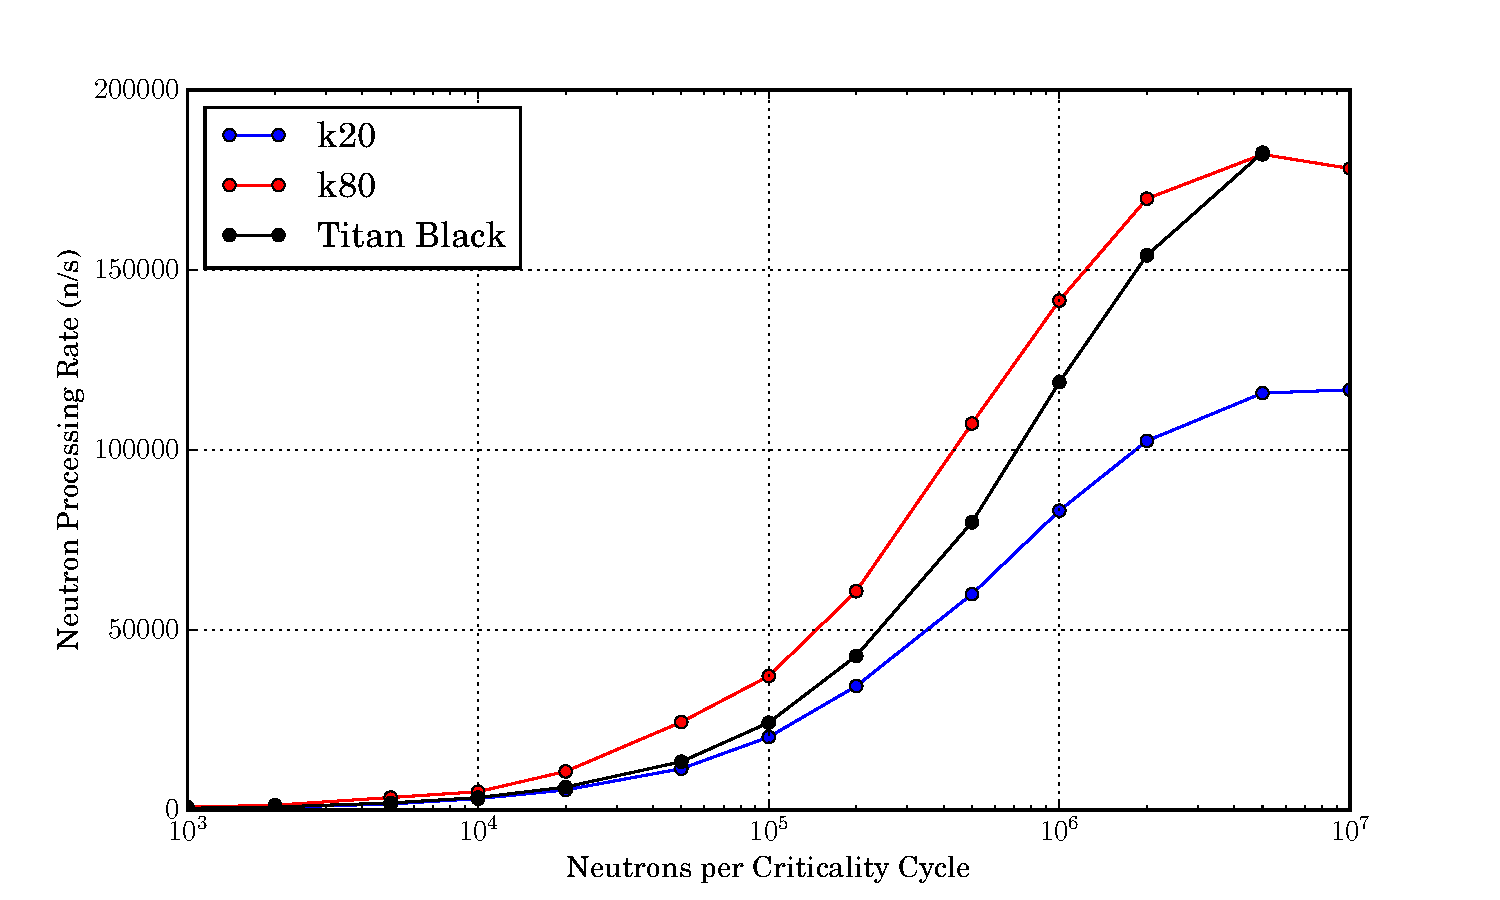
\includegraphics[width=0.8\textwidth,trim= 1cm 0cm 1cm 0cm]{graphics/scaling.pdf}
\caption{Neutron processing rate vs.\ number of neutrons per cycle for the hexagonal lattice test case. \label{scaling} }
\end{figure}

Performance increases until $5\times10^6$ neutrons per cycle, then flattens above this.  This curve was calculated using the hexagonal pin lattice test case, and may look different for different problems, but this number gives a rough estimate of where maximum performance occurs for WARP running on a Titan Black card.  This plot also shows ``tail effect''\textemdash that the processing rate decreases with the number of active neutrons in a cycle.  
% This is one example, do you have any incite into how this changes with problem size or complexity? Any sense of the boundaries of applicability? Should the user just do a couple of quick test runs to get a sense of this curve before running their real calculation? I feel like just a little more info would translate this into good advice :)


\subsection{Multiplication Factors}

Table \ref{results_table_keff} shows the multiplication factor deviations for the six criticality tests compared to MCNP 6.1 and Serpent 2.1.21 for WARP running on an NVIDIA Titan Black, K20, and K80 cards.  The ``$\Delta$MCNP'' row contains WARP's difference (in PCM) from MCNP, and the ``$\Delta$ Serpent'' row contains WARP's difference from Serpent.  These difference rows also contain $1\sigma$ and $2\sigma$ values that indicate the level at which the multiplication factors calculated by WARP agree with either Serpent or MCNP.  A ``y'' in the $1\sigma$ position indicates that the multiplcation factor values are mutually within 1 standard deviation of each other, i.e. e.g. the $\Delta \textrm{MCNP}<\sigma_{\textrm{MCNP}}+\sigma_{\textrm{WARP}}$.  This is the 90\% confidence interval and there is a 10\% probability that the the two codes could produce results outside of this interval.  The $2\sigma$ position is simply double the $1\sigma$ width and corresponds to the 99.8\% confidence interval (0.2\% chance of being outside).


\begin{table}[h]
\centering
\caption{The test case multiplication factors and runtimes for WARP using a Titan Black GPU versus those of Serpent 2.1.21 and MCNP 6.1.}
\label{results_table_keff}
\footnotesize
\begin{tabular}{| l | r | r | r |}
\cline{2-4}
\multicolumn{1}{c|}{}               & Jezebel                         &  Homogenized Block               & Pin Cell                          \\
\hline                          
Serpent 2.1.21                      & 0.9997840 $\pm$ 9.50E-5         & 0.5934090 $\pm$ 1.20E-4          & 0.2750510 $\pm$ 1.80E-4           \\
\hline                          
MCNP 6.1                            & 0.9999600 $\pm$ 7.00E-5         & 0.5933000 $\pm$ 4.00E-5          & 0.2752100 $\pm$ 4.00E-5           \\
\hline                          
WARP Titan Black                    & 1.0000620 $\pm$ 9.58E-5         & 0.5933724 $\pm$ 1.24E-4          & 0.2750294 $\pm$ 1.46E-4           \\
    \qquad\qquad   $\Delta$ Serpent & 27.80, $1\sigma$ n, $2\sigma$ y & -3.66, $1\sigma$ y, $2\sigma$ y  &  -2.16, $1\sigma$ y, $2\sigma$ y  \\
    \qquad\qquad   $\Delta$ MCNP    & 10.20, $1\sigma$ y, $2\sigma$ y &  7.24, $1\sigma$ y, $2\sigma$ y  & -18.06, $1\sigma$ n, $2\sigma$ n  \\
\hline
WARP K20                            & 1.0000212 $\pm$ 7.82E-5         & 0.5934539 $\pm$ 1.66E-4          & 0.2751048 $\pm$ 2.07E-4           \\
    \qquad\qquad   $\Delta$ Serpent & 23.72, $1\sigma$ n, $2\sigma$ y & 4.49 , $1\sigma$ y, $2\sigma$ y  &   5.38, $1\sigma$ y, $2\sigma$ y  \\
    \qquad\qquad   $\Delta$ MCNP    &  6.12, $1\sigma$ y, $2\sigma$ y & 15.39, $1\sigma$ n, $2\sigma$ y  & -10.52, $1\sigma$ n, $2\sigma$ y  \\
\hline
WARP K80                            & 0.9999602 $\pm$ 9.58E-5         & 0.5932266 $\pm$ 1.24E-4          & 0.2749884 $\pm$ 1.56E-4           \\
    \qquad\qquad   $\Delta$ Serpent & 17.62, $1\sigma$ y, $2\sigma$ y & -18.24, $1\sigma$ n, $2\sigma$ y &  -6.36, $1\sigma$ y, $2\sigma$ y  \\
    \qquad\qquad   $\Delta$ MCNP    &  0.02, $1\sigma$ y, $2\sigma$ y &  -7.34, $1\sigma$ y, $2\sigma$ y & -22.26, $1\sigma$ n, $2\sigma$ n  \\
\hline
\end{tabular}

\smallskip

\begin{tabular}{| l | r | r | r |}
\cline{2-4}
\multicolumn{1}{c|}{}               & FLiBe Cell                      & Sodium Pin Cell                  & Hex Assembly                      \\
\hline                       
Serpent 2.1.21                      & 0.8804900 $\pm$ 8.70E-5         & 1.0987100 $\pm$ 2.20E-4          & 1.0503300 $\pm$ 7.20E-5           \\
\hline                       
MCNP 6.1                            & 0.8805100 $\pm$ 6.00E-5         & 1.0987700 $\pm$ 6.00E-5          & 1.0499500 $\pm$ 7.00E-5           \\
\hline                       
WARP Titan Black                    & 0.8807005 $\pm$ 9.58E-5         & 1.0986860 $\pm$ 7.82E-5          & 1.0510795 $\pm$ 9.58E-5           \\
    \qquad\qquad   $\Delta$ Serpent & 21.05, $1\sigma$ n, $2\sigma$ y & -2.40, $1\sigma$ y, $2\sigma$ y  &  74.95, $1\sigma$ n, $2\sigma$ n  \\
    \qquad\qquad   $\Delta$ MCNP    & 19.05, $1\sigma$ n, $2\sigma$ y & -8.40, $1\sigma$ y, $2\sigma$ y  & 112.95, $1\sigma$ n, $2\sigma$ n  \\
\hline
WARP K20                            & 0.8807086 $\pm$ 9.58E-5         & 1.0987912 $\pm$ 5.53E-5          & 1.0510620 $\pm$ 9.58E-5           \\
    \qquad\qquad   $\Delta$ Serpent & 21.86, $1\sigma$ n, $2\sigma$ y & 8.12, $1\sigma$ y, $2\sigma$ y   &  73.20, $1\sigma$ n, $2\sigma$ n  \\
    \qquad\qquad   $\Delta$ MCNP    & 19.86, $1\sigma$ n, $2\sigma$ y & 2.12, $1\sigma$ y, $2\sigma$ y   & 111.20, $1\sigma$ n, $2\sigma$ n  \\
\hline
WARP K80                            & 0.8807546 $\pm$ 9.58E-5         & 1.0985898 $\pm$ 5.53E-5          & 1.0511035 $\pm$ 1.24E-4          \\
    \qquad\qquad   $\Delta$ Serpent & 26.56, $1\sigma$ n, $2\sigma$ y & -12.02, $1\sigma$ y, $2\sigma$ y &  77.35, $1\sigma$ n, $2\sigma$ n  \\
    \qquad\qquad   $\Delta$ MCNP    & 24.56, $1\sigma$ n, $2\sigma$ y & -18.02, $1\sigma$ y, $2\sigma$ y & 115.35, $1\sigma$ n, $2\sigma$ n  \\
\hline
\end{tabular}
\end{table}


From Table \ref{results_table_keff}, it can be seen that WARP agrees with either MCNP \emph{or} Serpent (they sometimes do not exactly agree with each other!) on the $1\sigma$ level for all cases except the FliBe cell and the hex assembly cases.  The FliBe cell case agrees on the $2\sigma$ level, but the hex assembly case does not, indicating that there is a problem with the way WARP is solving the hex assembly case.  Speculation on what could be casuing this is discussed in Section \ref{sec:disc}.

\subsection{Runtimes}


Table \ref{results_table_times} shows the transport cycle runtimes for the six criticality tests compared to MCNP 6.1 and Serpent 2.1.21 for WARP running on an NVIDIA Titan Black, K20, and K80 cards.  The values in the time rows are reported in minutes.  The ``$\Delta$ MCNP'' row contains WARP's speedup factor over MCNP, and the ``$\Delta$ Serpent'' row contains WARP's speedup factor over Serpent.


\begin{table}[h]
\centering
\caption{The test case transport cycle run times (in minutes) for WARP, Serpent 2.1.21, and MCNP 6.1.  Values in the ``$\Delta$'' rows contain the speedup factor of WARP compared the the corresponding production code running on a Berkelium PSSC node and a SAVIO2 node.}
\label{results_table_times}
\footnotesize
\begin{tabular}{| l r | r | r | r |}
\cline{3-5}
\multicolumn{2}{c|}{}                            & Jezebel     & Homogenized Block & Pin Cell     \\
\hline                          
Serpent 2.1.21   &    Bk PSSC                    & 7.24        & 39.41             & 146.15       \\
                 &    SAVIO2                     & 6.32        & 24.10             & 76.51        \\
\hline                                        
MCNP 6.1         &    Bk PSSC                    &  30.57      & 98.40             & 131.27       \\
                 &    SAVIO2                     &   4.95      & 44.03             & 64.18        \\
\hline                          
\multicolumn{2}{|l|}{WARP Titan Black}           &  1.47       & 7.53              &  26.47       \\
\multicolumn{2}{|r|}{$\Delta$ Serpent (bk, s2)}  & 4.91  4.29  & 5.23  3.20        &  5.52  2.89  \\
\multicolumn{2}{|r|}{$\Delta$ MCNP    (bk, s2)}  & 20.74 3.36  & 13.07 5.85        &  4.96  2.42  \\
\hline
\multicolumn{2}{|l|}{WARP K20}                   & 2.45         & 12.60            & 42.55        \\
\multicolumn{2}{|r|}{$\Delta$ Serpent (bk, s2)}  & 2.96  2.58   & 3.13  1.91       & 3.44  1.80   \\
\multicolumn{2}{|r|}{$\Delta$ MCNP    (bk, s2)}  & 12.49 2.02   & 7.81  3.50       & 3.09  1.51   \\
\hline
\multicolumn{2}{|l|}{WARP K80}                   & 1.18         & 5.79             & 20.91        \\
\multicolumn{2}{|r|}{$\Delta$ Serpent (bk, s2)}  & 6.11  5.34   & 6.81  4.17       & 6.99  3.66   \\
\multicolumn{2}{|r|}{$\Delta$ MCNP    (bk, s2)}  & 25.80 4.18   & 17.01 7.61       & 6.28  3.07   \\
\hline
\end{tabular}

\smallskip

\begin{tabular}{| l r | r | r | r |}
\cline{3-5}
\multicolumn{2}{c|}{}                            & FLiBe Cell   & Sodium Pin Cell & Hex Assembly  \\
\hline                                    
Serpent 2.1.21   &   Bk PSSC                     & 79.16        & 120.86          & 81.54         \\
                 &   SAVIO2                      & 45.08        &  68.46          &  44.32        \\
\hline                                        
MCNP 6.1         &   Bk PSSC                     & 269.47       & 320.40          & 160.68        \\
                 &   SAVIO2                      & 81.03        & 199.15          & 112.25        \\
\hline                       
\multicolumn{2}{|l|}{WARP Titan Black }          &  25.78       & 81.18           & 34.91         \\
\multicolumn{2}{|r|}{$\Delta$ Serpent (Bk, S2)}  &  3.07  1.75  & 1.49  0.84      & 2.34  1.27    \\
\multicolumn{2}{|r|}{$\Delta$ MCNP    (Bk, S2)}  &  10.45 3.14  & 3.95  2.45      & 4.60  3.22    \\
\hline
\multicolumn{2}{|l|}{WARP K20 }                  & 39.83        & 121.34          & 56.03         \\
\multicolumn{2}{|r|}{$\Delta$ Serpent (Bk, S2)}  &  1.99  1.13  & 1.00  0.56      & 1.46  0.79    \\
\multicolumn{2}{|r|}{$\Delta$ MCNP    (Bk, S2)}  &  6.77  2.03  & 2.64  1.64      & 2.87  2.00    \\
\hline
\multicolumn{2}{|l|}{WARP K80   }                & 24.68        & 81.40           & 35.63         \\
\multicolumn{2}{|r|}{$\Delta$ Serpent (Bk, S2)}  & 3.21  1.83   &  1.48  0.84     &  2.29  1.24   \\
\multicolumn{2}{|r|}{$\Delta$ MCNP    (Bk, S2)}  & 10.92 3.28   &  3.94  2.45     &  4.51  3.15   \\
\hline
\end{tabular}
\end{table}


It can be seen from Table \ref{results_table_times} that WARP runs fastest on the K80 card both Serpent and MCNP run fastest on the SAVIO2 node.  This makes sense since these are the two newest pieces of hardware considered in the tests.  It is important to note that the Titan Black card performs almost as well as the K80 card, however.  Comparing the K80 card to a SAVIO2 node (the most relevant comparison), WARP runs 0.84 to 5.34 times as fast as Serpent and 2.45 to 7.61 times as fast as MCNP.   The largest speedup over Serpent is for the Jezebel test, the largest speedup over MCNP is for the homogenized block test, and the smallest speedup is for the sodium pin cell test compared to both Serpent and MCNP.  This speedup factor is calculated over an entire compute node, so these cards can have performance equivalent to 0.84 to 7.61 compute nodes, depending on the type of simulation considered.  For the sodium pin case, where there is relatively a lot of cross section processing, a SAVIO2 node running Serpent actually performs better than WARP on a K80 card.  For problems where there is less cross section processing (higher geometry processing fraction), WARP tend to perform better than a SAVIO2 node running Serpent.  WARP always performs better than a SAVIO2 node running MCNP, even with relatively heavy cross section processing, but this isn't a great surprise considering that MCNP doesn't use a unionized energy grid structure when processing cross sections.


\subsection{Spectra}

In the following subsections, spectra caluclated by WARP are compared to those calculated by Serpent and MCNP for identical gemetries and materials.  Every spectrum is binned into 1024 equi-log bins from $10^{-11}$ to $20$ MeV.  In tests where there is a large region of little to no flux (like in the fast spectrum inside the Jezebel sphere), the energy bin structure is not changed, but the energy range of the plot is limited to the region where there is nonzero flux.  The relative difference compared to the MCNP spectrum is shown in the top subplot below the main spectrum plot, and the relative difference from the Serpent spectrum is shown in the lower subplot.  The green shaded area in the error subplots shows the space within 2 standard devitions of the statistical uncertainty of the production code.  Unlike the intervals reported previous subsection, the interval shown in green is only for the production code results.  In other words, the codes should have results within the 2$\sigma$ interval 95.45\% of the time (as opposed to 99.8\% of the time).

%%%%%
\newpage
\subsubsection{Test 1 - ``Jezebel'' Bare Pu Sphere}

Figure \ref{jezebel_spec} shows the volume-averaged flux spectrum in the Jezebel sphere.  The relative difference of WARP compared to Serpent and MCNP is very low, with the normalized tally bins being less than 0.5\% from each other in regions where the flux is large.  Of course, when the flux is small, the statistical uncertainty becomes much higher, and the relative difference becomes noisy.   The relative error is almost always inside the 2$\sigma$ confidence interval as well, indicating that the simulations are statistically identical. 

\begin{figure}[h!]
\centering
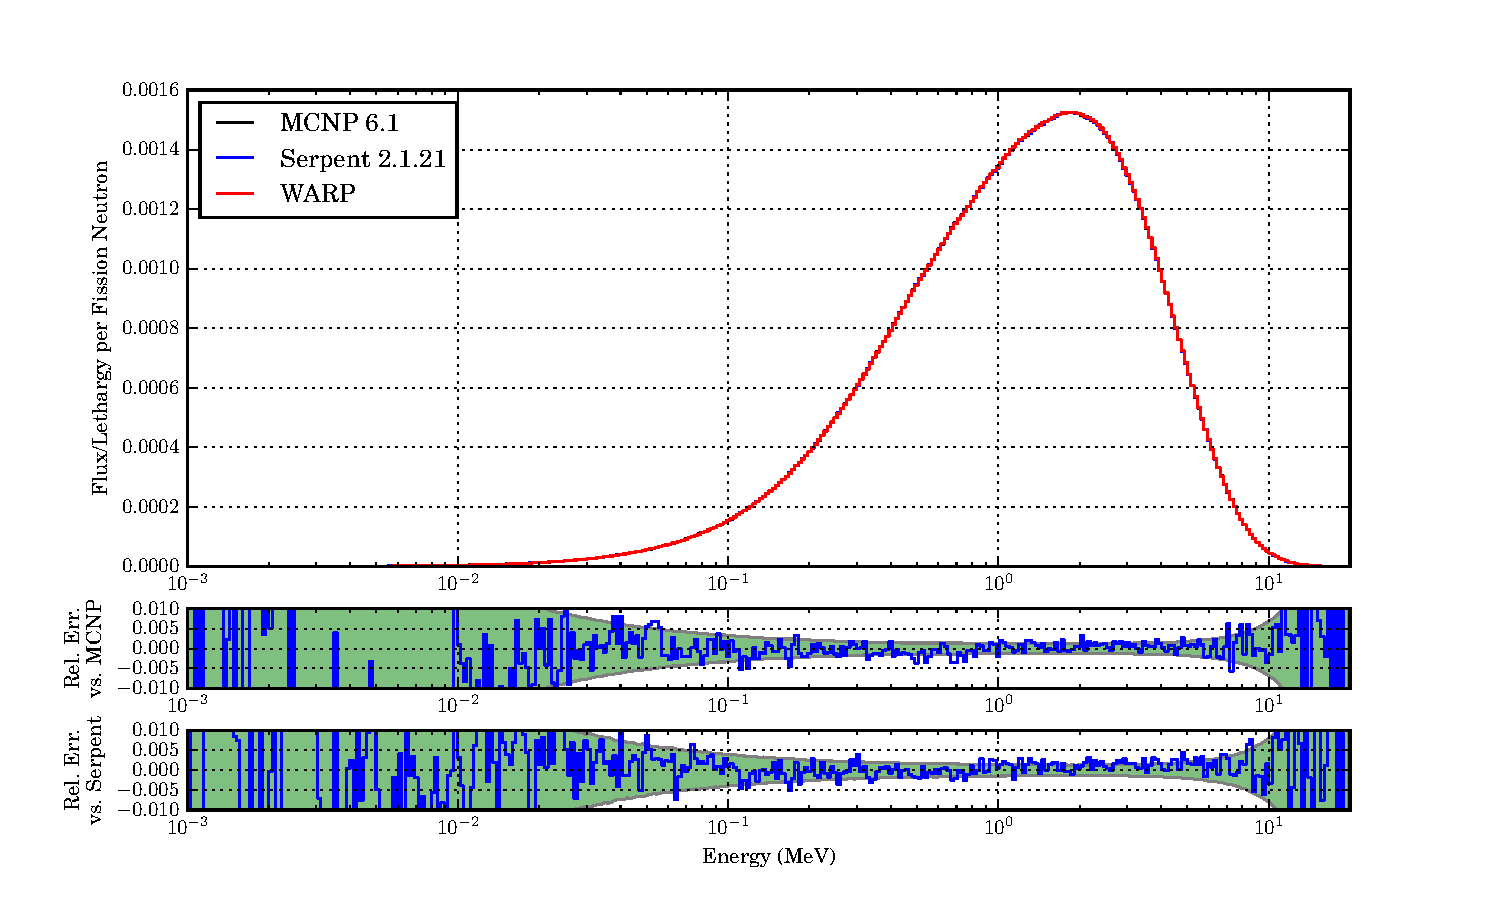
\includegraphics[width=0.9\textwidth,trim= 1cm 0cm 1cm 0cm]{graphics/jezebel_spec.pdf}
\caption{Volume-averaged flux spectra inside the sphere of the Jezebel test case. \label{jezebel_spec} }
\end{figure}

%%%%%
\newpage
\subsubsection{Test 2 - Homogenized Fuel Block}

Figure \ref{homfuel_spec} shows the volume-averaged flux spectrum in the homogenized fuel block.  The relative difference compared to MCNP and Serpent is again shown in the lower subplots.  The relative difference compared to MCNP again generally less than 0.15\% and appears to have a zero mean, but the error compared to Serpent has a constant positive offset, indicating a slightly different normalization.  This kind of offset appears in other spectra as well but only when comparing to Serpent.  This indicates a possible normalization discrepency between MCNP and Serpent.  There also appears to be some  deviations with similar structure from 0.1 to 0.3 MeV, indicating that some kind of reaction sampling may not be treated exactly the same way as in Serpent and MCNP.

% you might want to say how it differs from serpent as well to give a hint about which normalization might be more correct. The current comparison feels incomplete.

\begin{figure}[h!]
\centering
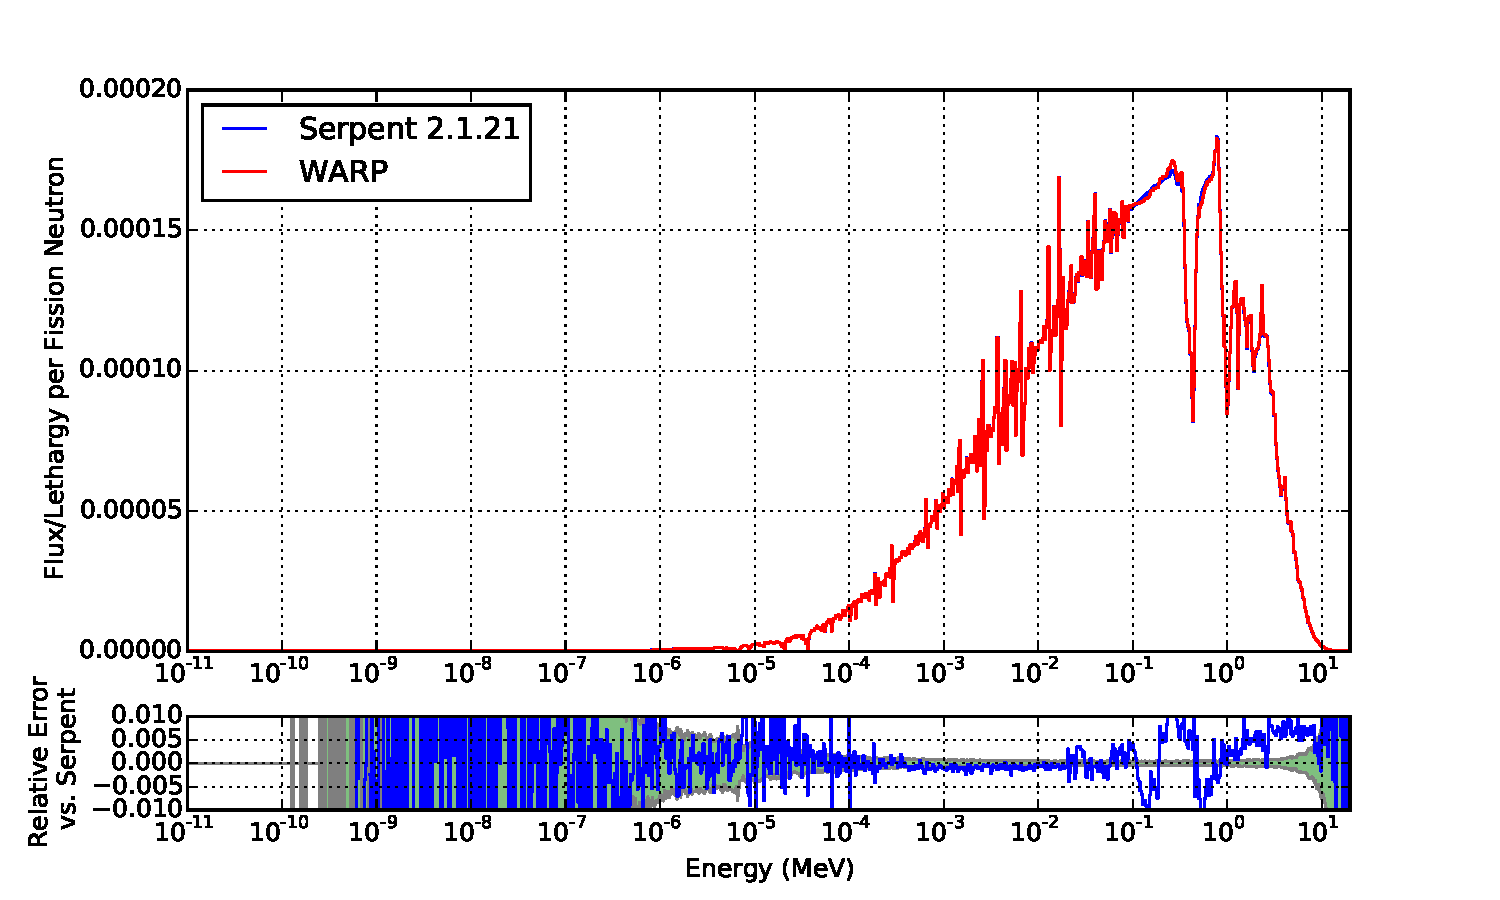
\includegraphics[width=0.9\textwidth,trim= 1cm 0cm 1cm 0cm]{graphics/homfuel_spec.pdf}
\caption{Volume-averaged flux spectra inside the homogenized fuel block. \label{homfuel_spec} }
\end{figure}

%%%%%
\newpage
\subsubsection{Test 3 - Zr-Clad UO$_2$ Pin in Heavy Water}

Figure \ref{pincell_spec} shows the volume-averaged flux spectrum inside the fuel rod in the Zr-clad UO$_2$ pin in heavy water test case.  Again, the relative difference is generally less than 1\% where the flux is large.  Compared to Serpent, the WARP spectrum again appears to have a small constant offset.  The entire energy range agrees well with MCNP, however, indicating that all the reaction laws were processed indenctically to MCNP for the nuclides present in this test case.


\begin{figure}[h!]
\centering
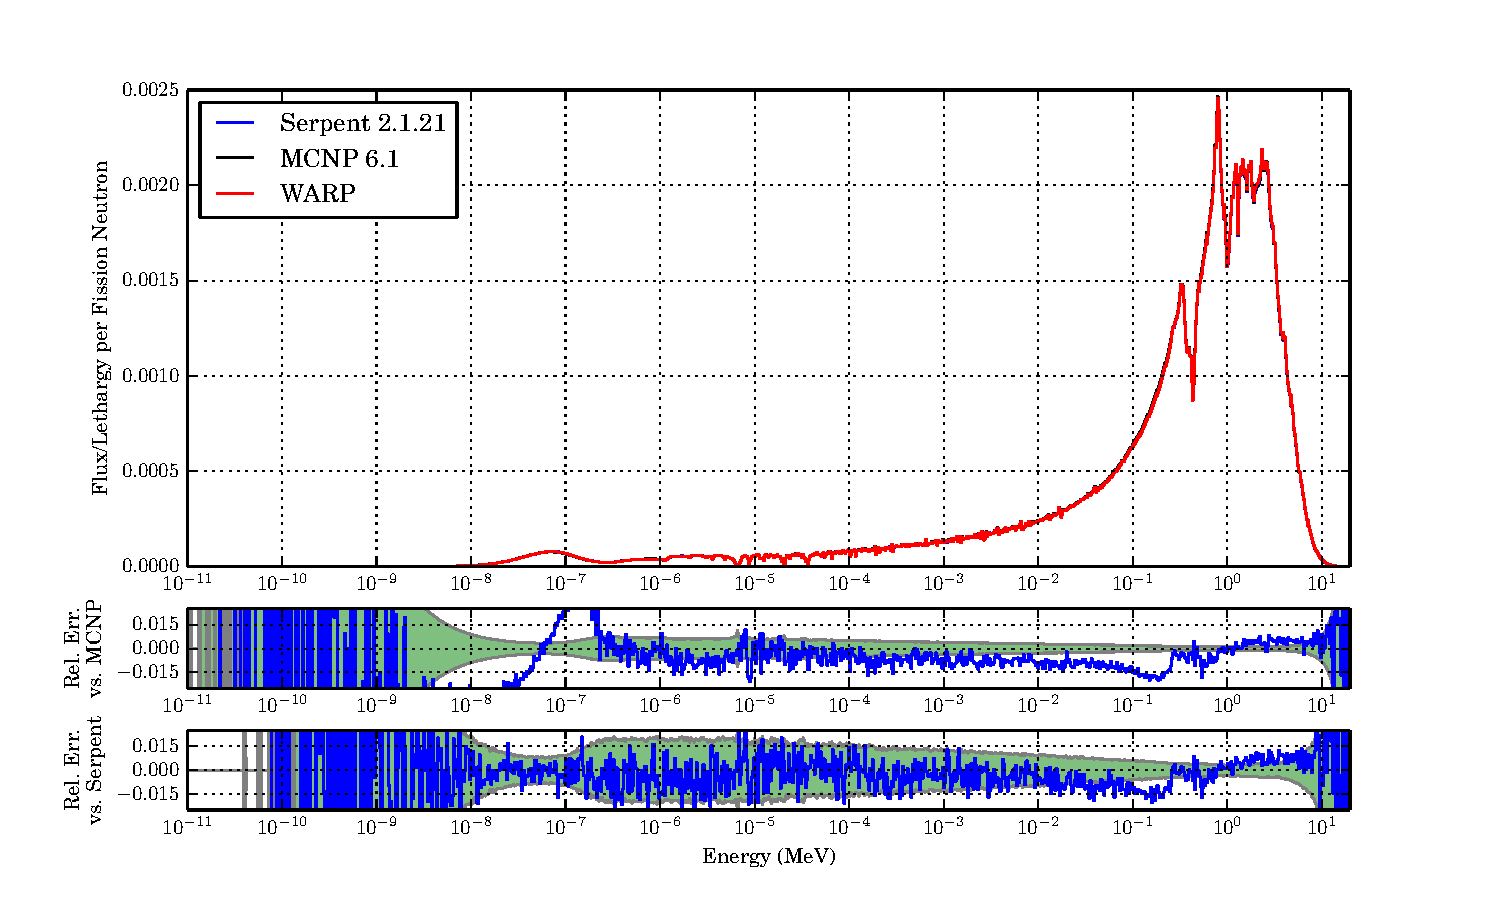
\includegraphics[width=0.9\textwidth,trim= 1cm 0cm 1cm 0cm]{graphics/pincell_spec.pdf}
\caption{Volume-averaged flux spectra inside the oxide fuel of the Zr-clad pin in heavy test case \label{pincell_spec} }
\end{figure}

%%%%%
\newpage
\subsubsection{Test 4 - Homogenized Fuel Pebble in FLiBe}

Figure \ref{flibe_spec} shows the volume-averaged flux spectrum in the fuel pebble for the reflective FLiBe test case.  Here, the relative difference is generally less than 0.1\% where the flux is large.  The WARP spectrum again has a constant offset compared to the Serpent spectrum, but compares well to MCNP apart from the significant deviations around large resonances in the 20 keV to 1 MeV range.  This again highlights that there is probably a reaction law that isn't processed identically to MCNP.

\begin{figure}[h!]
\centering
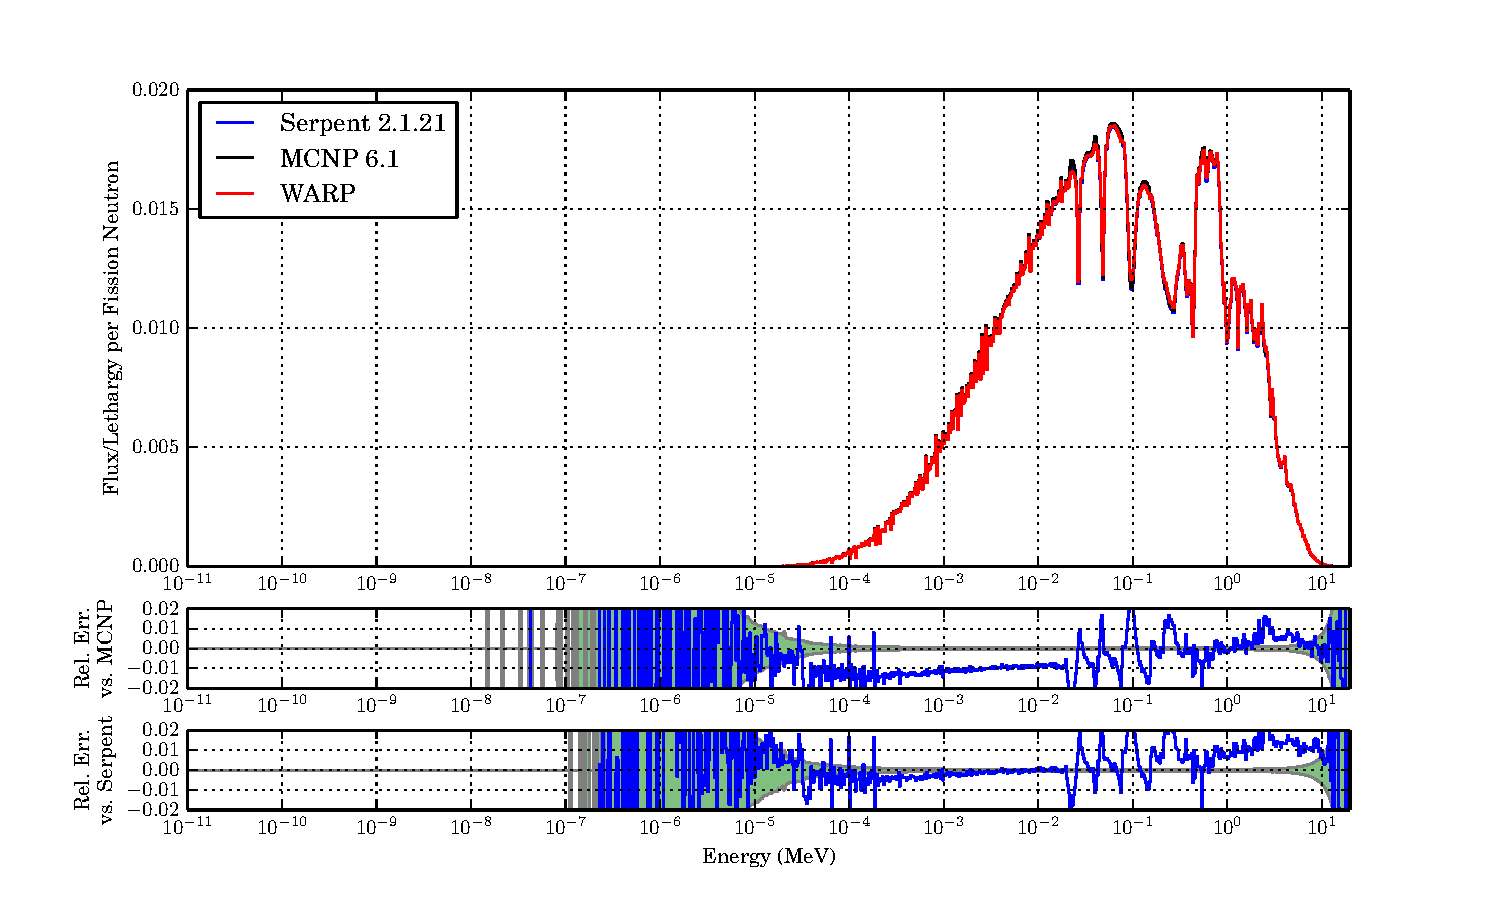
\includegraphics[width=0.9\textwidth,trim= 1cm 0cm 1cm 0cm]{graphics/flibe_spec.pdf}
\caption{Volume-averaged flux spectra inside the fuel pebble of the reflective FLiBe test case. \label{flibe_spec} }
\end{figure}

%%%%%
\newpage
\subsubsection{Test 5 - Stainless Steel Clad Metallic Uranium Pin in Liquid Sodium}

Figure \ref{sodiumpin_spec} shows the volume-averaged flux spectrum in the fuel for the reflective sodium cooled, steel clad, metallic fuel test case.  The relative difference is generally less than 0.1\% where the flux is large.  The WARP spectrum again has a constant offset compared to the Serpent spectrum, but compares well to MCNP apart from the significant deviations around large resonances in the 20 keV to 1 MeV range.  This again highlights that there is probably a reaction law that isn't processed identically to MCNP.

\begin{figure}[h!]
\centering
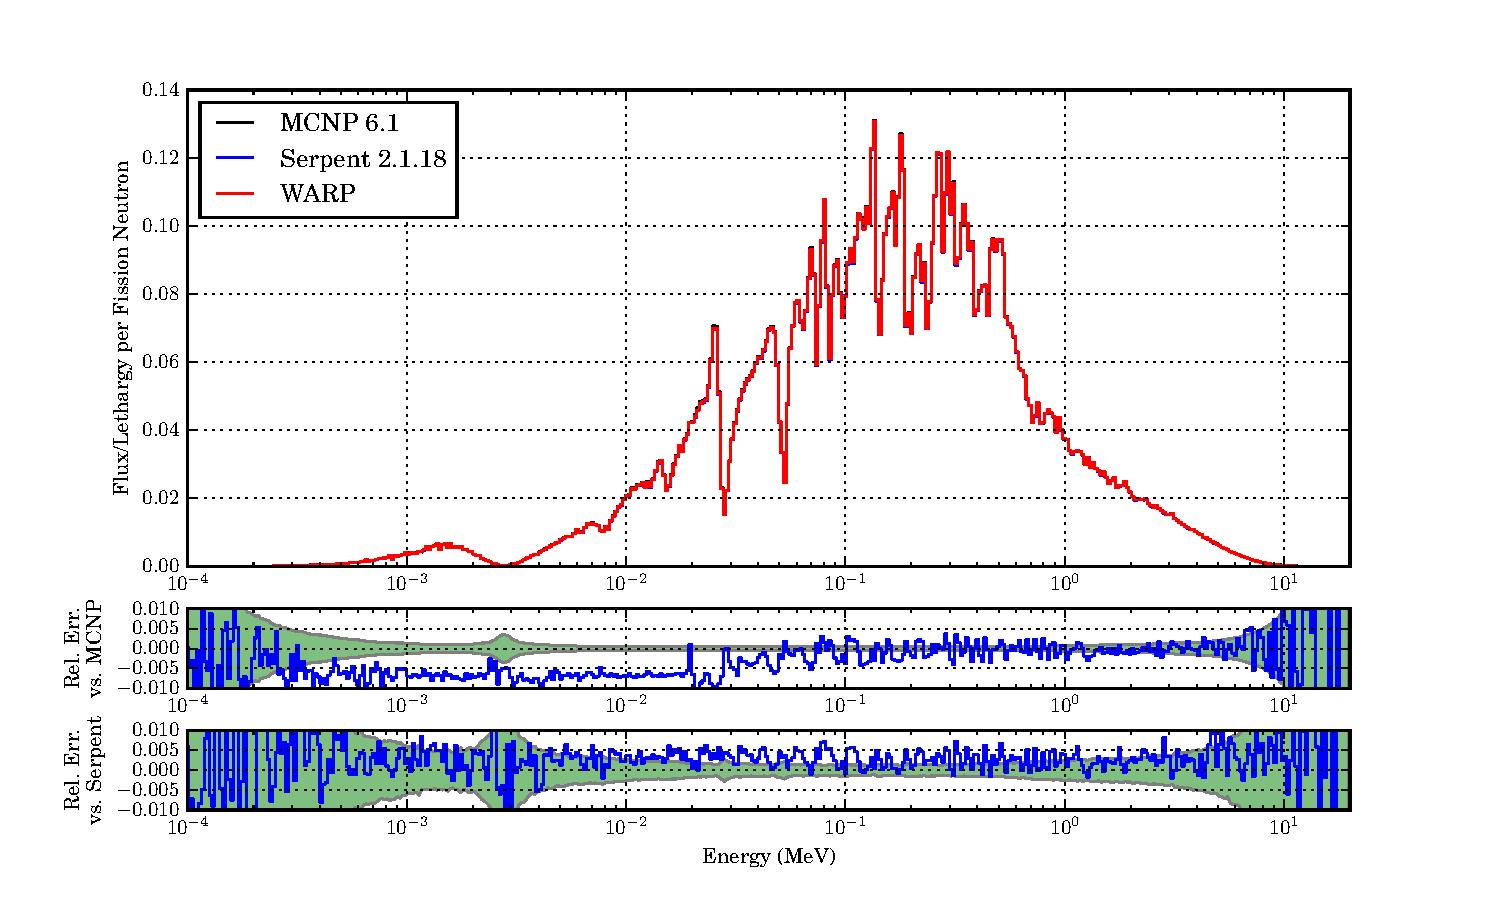
\includegraphics[width=0.9\textwidth,trim= 1cm 0cm 1cm 0cm]{graphics/sodiumpin_spec.pdf}
\caption{Volume-averaged flux spectra inside the fuel of the reflective, steel clad, sodium cooled pin test case. \label{sodiumpin_spec} }
\end{figure}


%%%%%
\newpage
\subsubsection{Test 6 - Zr-Clad Hexagonal UO$_2$ Pin Cell Lattice in Light Water}

Figure \ref{assembly-lw_spec} shows the volume-averaged flux spectrum in the center pin of the Zr-clad hexagonal oxide fuel pin lattice in light water test case. The relative difference is generally less than 5\% where the flux is large, but this time the WARP results are always within the statistical error of both MCNP and Serpent.  There is no constant offset compared to Serpent or MCNP and no large devisions, indicating that all the reaction laws were processed indenctically to both Serpent and MCNP for the nuclides present in this test case.  This is also the only test case other than Jezebel where MCNP and Serpent give identical spectra.

\begin{figure}[h!]
\centering
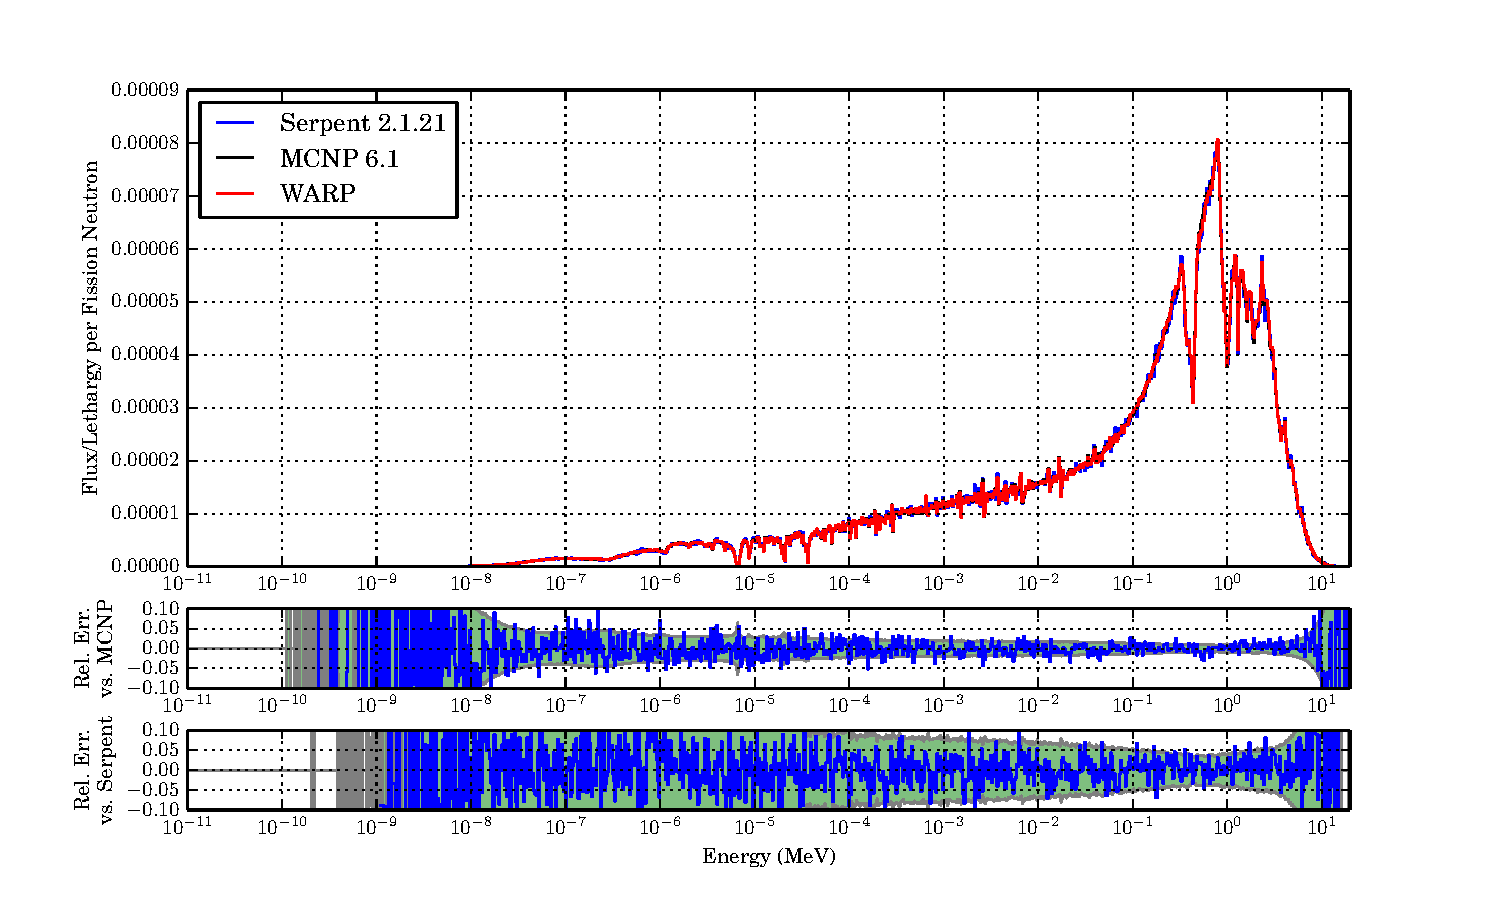
\includegraphics[width=0.9\textwidth,trim= 1cm 0cm 1cm 0cm]{graphics/assembly-lw_spec.pdf}
\caption{Volume-averaged flux spectra inside the center fuel pin of the hexagonal pin lattice test case. \label{assembly-lw_spec} }
\end{figure}


\subsection{History Power}

For productivity, the ``history power,'' or  number of neutron histories a system can process per unit time, is of primary interest when deciding what kind of system to purchase since it determines how quickly results can be produced.  In addition to this, the history power per harware cost is of interest for initial capital investment, and the history power per unit energy are of interest for operational costs.  Table \ref{history_power} shows the history power (neutron histories per second) and relative costs of GPU system running WARP compared to MCNP and Serpent running on a the aforementioned CPU platforms.  The history powers shown in Table \ref{history_power} were calculated by summing the total number of neutron processed in all six test cases and dividing this number by the sum of the run times of the six cases for each code/platform combination (i.e. $3.9\times10^8 / \textrm{sum of run times}$).  This way, the average is not biased towards a special case that allows a code to process neutrons especially fast.  The history power per capital is simply the averaged neutron processing rate divided by the hardware cost of the plotform.  The history power per watt is similar, except divided by the platform's total maximum electrical power consumption rather than the cost.  The costs and electrica powers used are shown in Table \ref{platform_table}.

\begin{table}[h]
\centering
\caption{The history power and costs of performing Monte Carlo neutron transport on GPU and CPU systems.}
\label{history_power}
\small
\begin{tabular}{| l r | r | r | r |}
\cline{3-5}
\multicolumn{2}{c|}{}             & H. Power   & H.P. / Capital   & H.P. / Watt  \\
\hline                            
Serpent 2.1.21   &   Bk PSSC      & 2.32E+6    &   249           &  5,033        \\
                 &   SAVIO2       & 8.84E+6    & 1,305           & 42,082        \\
\hline                                 
MCNP 6.1         &   Bk PSSC      & 2.32E+6    &   249           &  5,033        \\
                 &   SAVIO2       & 4.63E+6    &   684           & 22,039        \\
\hline                            
WARP             &   Titan Black  & 1.32E+7    & 8,675           & 52,778        \\
                 &   K20          & 8.52E+6    & 2,561           & 37,847        \\
                 &   K80          & 1.38E+7    & 2,760           & 45,995        \\
\hline
\end{tabular}
\end{table}


Table \ref{history_power} shows that, on average, for the test cases considered, a new NVIDIA GPU card can process neutrons about 1.6 times as fast as a new multiprocessor/multicore CPU node running Serpent and about 3 times as fast as a CPU node running MCNP.  From a capital investment standpoint, the a K80 card costs about half as much as a SAVIO2 node per neutron processing power and consumes about the same amount of electricity.  The Titan Black, however, performs about as well as a K80 from the neutron processing rate standpoint, but costs about a third as much and consumes 20\% less electricity.  Since WARP uses single-precision data and math in order to fully exploit the capacities available on consumer GPUs (like the Titan Black), the capital and electrical costs of running WARP can be greatly reduced.  


%%%%%%%%%%%%%%%%%%%
%%%%%%%%%%%%%%%%%%%
%%%%%%%%%%%%%%%%%%%

\section{Discussion}
\label{sec:disc}

The differences seen in the multiplcation factors and spectra calculated by WARP compared to those calculated by Serpent and MCNP are most likely due to a reaction law being inexactly processed.  Whether this is due to a bug or if it has to do with single precision math has not been determined.  Some laws potentiall require division by small numbers and comparing and/or adding the result to other numbers.  Roundoff error from single precision math could make these operations inaccurate and ultimately lead to visible differences in the neutron spectrum and multiplcation factor.  

Monte Carlo is a great place to take advantage of single precision math since solution convergence does not normally depend on derivatives, except potentially in cross section processing law, and the major places roundoff error can affect the solution is in tally accumulation and cross section processing.  Currently, WARP calculates the total macroscopic cross section of a material on the fly, and roundoff could become a problem around resonancese where the cross section of one nuclide (or several) is much larger than the that of the other nuclides in the material.  In this case, the additions from the relatively small cross section nuclides could be neglected and could lead to oversampling their reactions in the subsequent routines (since the material's calculated total macroscopic cross section would be smaller than it should be).  This problem could be circumvented by preprocessing the material's total macroscopic cross section using double precision math on the host before the data is given to the GPU as single precision numbers at the cost of increasing the memory footprint.

Anotherr place roundoff error could casue problems is in tally accumulation.  WARP calculates the flux in a cell by calculating the inverse of the macroscopic cross section at a collision site by adding it to the sum of all previous collisions.  If a large resonance lies within an energy bin, very dissimilar values could be added together and precision could be lost.  This could be cicumvented by using double precision data for the tally arrays.  The cost of doing so would have to be measured, but hopefully it would be small since tally accumulation only happens once per transport cycle and is therefore a relatively infrequent operation.

WARP uses integer math to calculate multiplication factors.  Long intereger values are stored on the host for the total number of fissions producded in a simulation, and integer yield values are accumulated into it after each batch.  At the end of the simulation, the long integer value containting the total number of fission neutrons produced in the entire simulation is divided by the total number of source neutrons run, yielding the final value for the multiplication factor. Since integer math is used during this whole process, roundoff error from accumulation can not affect it as long as overflow doesn't occur (hence using the long interger data type)  Roundoff error in the reaction selection and processing routines could affect the individual yield values and their frequency, however.

It is worht noting that MCNP and Serpent calculated somewhere different solutions in these studies, which shows that getting exactly the same answer is quiter difficult since each code handles things slightly differently.  This makes it difficult to know what is really correct, but as long as the solutions are under an acceptable error level compared to what can be detected in the physical world, we should all be satisfied.  The potential niche use for WARP would be to do cheap and fast calculations where large total throughput is needed, not precision.  Using a large parametric study as an example, once an optimial region has been found in the parameter space, WARP's job would be done.  This knowledge could then be used as a starting point for more precise calculations with CPU codes.


%%%%%%%%%%%%%%%%%%%
%%%%%%%%%%%%%%%%%%%
%%%%%%%%%%%%%%%%%%%

\section{Conclusions}
\label{sec:conc}

It has been shown that WARP is able to perform high-fidelity neutron transport on GPUs.  Depending on the problem type and the card used, WARP can achieve performance equivalent to that of 2 to 13 CPU nodes with 4 AMD Opteron 6172 processors (48 cores) each.  The low capital and electrical cost of GPU platforms then lead to at least an order of magnitude more histories calculated per dollar spent.  This figure clearly shows that GPUs can be  very cost effective for continuous energy Monte Carlo neutron transport.

mention the rounding suspicion for the resonances.

The development of WARP has led to important conclusions regarding how to conduct neutron transport on GPUs as well, mainly that running with large datasets, and therefore a large number of threads, is important for good performance.  It was found that in the hexagonal lattice test case, maximum performance was achieved at $5\times10^6$ neutrons per criticality cycle.  It is important to keep the GPU saturated with threads so it can effectively pipeline data loads and issue instructions.  
% This conclusion doesn't seem to reflect what was discussed/presented above. This wasn't highlighted at all.
% Also, you changed the geometry routine but don't talk about how that has had an impact, or if you've measured the impact at all. Is there a comparison of WARP timing and memory use with the old geometry routine compared to the new one? That seems like it would be a really useful addition... 

WARP still has some bugs, as evidenced by the uniform deviation of the multiplication factors compared to MCNP/Serpent and the deviations apparent in the calculated spectra.  A large part of future development will be tracking them down to ensure that accurate results are produced.

WARP will be released as open source software, pending DOE approval, at \url{http://github.com/weft}. The ``warp'' is the high-tension, longitudinal thread in a weave of cloth, whereas the ``weft'' is the low tension, transverse thread.  On a loom, the warp threads are all moved in sync, then the weft is passed through them.  Naming the repository for the single thread that defines the phase of the warp seemed appropriate.
% love it!

%%%%%%%%%%%%%%%%%%%
%%%%%%%%%%%%%%%%%%%
%%%%%%%%%%%%%%%%%%%
\section{Future Development}
\label{sec:dev}

The initial goals of WARP have been completed, but there is much work still to be done if it is going to be of real use to the nuclear engineering community.  Basic functionality is currently good enough to assure the GPUs can accelerate high-fidelity Monte Carlo neutron transport calculations, but many capabilities need to be expanded and ensured to scale well to large numbers of neutrons, isotopes, and geometric zones.  
% You might want to spend the rest of the paragraph previewing what you will talk about in the rest of this section so we have a roadmap before entering it. 

Reproducibility of results when using the same random number seeds will also be investigated to ensure consistent results can be produced and that there are no systematic errors present in WARP.  Ensuring reproducibility will also be necessary in making a test suite for WARP, so future users can have confidence in their results and future developers can know their modifications do not introduce new errors into WARP.

The geometry is currently handled by OptiX, which provides a convenient way to obtain high-performance results, but OptiX had to be coerced into providing WARP with the information it needed, namely the material number via the point-in-polygon (PIP) algorithm.  The way OptiX executes this algorithm is not efficient since it must be done iteratively using OptiX's native functions instead of calculating the ordered list of intersections in a single trace.  NVIDIA is releasing ``OptiX Prime'' with OptiX 3.5 \cite{optix3.5}, which promises to provide a more ``to the metal'' ray tracing experience, and might be leveraged to provide more efficient single-traverse functionality.  OptiX could also be replaced by Rayforce \cite{rayforce}, a high-performance GPU ray tracing library developed by VSL that has this functionality built-in and is currently available free of charge for noncommercial use.

%grid thinning?

The geometry routines could also be replaced by handwritten routines that use combinatorial solid geometry like Serpent and MCNP.  This would make writing input for WARP more like what most nuclear engineers are already used to and, more importantly, could provide a potential performance increase.  A universe-based CSG representation may map very well to the GPU and may even be able to fit inside of shared memory for small numbers of surfaces.  Using an efficient CSG method would further lend itself to using Woodcock delta-tracking for the neutrons and thus getting rid of the tracing algorithms and libraries altogether.   
%The new PIP algorithm uses surface sense in order to eliminate a surface hit list and greatly improves the scalability of WARP's geometry routines, and in this way is like a hybrid CSG and ray tracing algorithm. 
% again, there isn't any evidence provided that shows the impact of the new geometry routine.
% The new algorithm uses OptiX to determine which surfaces lie along a flight path, then calculates the surface normals to determine if a neutron is nested in the cell or not.

WARP's execution can also be improved.  The amount of memory required per neutron was not tracked in this initial development, much less optimized, since developing a functioning code was the main priority.  Reducing the memory needed per neutron would be highly beneficial in the sense that more concurrent neutrons could be launched using the reclaimed memory space.  Dynamic parallelism can be implemented to minimize kernel launch overhead and host-device communication in the inner transport loop.  Dynamic parallelism is a feature introduced into the NVIDA Kepler GPUs that allows kernels to be launched from kernels, and could eliminate the host needing to contain the main transport loop.  Neither CUDPP nor OptiX support its use, however.  CUDPP could be replaced with newer, higher-performance libraries (e.g.\ CUB) that do support dynamic parallelism, but OptiX would have to be replaced by a handwritten kernel to perform the necessary geometric tasks.  Textures could be thoroughly investigated as they might provide better performance in tasks where their free linear interpolation and spatial caching could provide a performance boost, like in an energy grid search on a tree structure.   Alternatively, using optimized graph search libraries, such as ``gunrock,'' could be used to perform the energy grid search \cite{gunrock}.

%WARP also currently only supports fixed-source mode in the non-remapping version as it requires popping secondary neutrons back into the active neutron pool after every iteration of the inner transport loop.  This operation is expensive since it is a global operation that must be done often.  This algorithm could be changed to be more like a criticality run, where the primary neutrons are all transported together, then the next (smaller) generation of secondary particles are transported, then the next, and so on.  This way, the pop routine is only executed in the outer loop, and could produce faster results.  

WARP suffers from ``tail effect,'' where performance drops off as the number of active neutrons decreases.  Developing a method that keeps the active neutron number high would greatly improve performance, but could become quite complicated as generations would start to overlap and calculation of the multiplication factor couldn't be done in between cycles  as it is now.  Multi-GPU support should also be added so that WARP can be used effectively on computers with more than one GPU.

If an entire overhaul of the WARP transport algorithm is feasible, using a streaming multiprocessor (SM)-based algorithm might be investigated for replacing the current global one.  This type of algorithm would treat each SM as an independent processor and would provide each a bank of neutrons to transport, as is done by Liu and Henderson \cite{tianyu,henderson}.   This way, neutron data could be stored in very fast shared memory, but using this memory space would compete with storing geometric information there.  Also, since a smaller set of neutrons could be stored, the SMs would need to communicate to determine which of the next neutrons they would take out of the global bank, or they would need to periodically rendezvous to shared source information and ensure that the distributions they use are each converged.  This type of transport algorithm would also preclude using OptiX, since it does not have SM-level functionality \cite{optix}.

Since global memory comes at a premium on GPUs, an on-the-fly temperature treatment for nuclides would likely be required if more than a handful of isotopes are desired at more than one temperature.  Methods like those used in Serpent could be adapted for use on the GPU \cite{serpent}.  On-the-fly methods reduce the amount of storage needed, but they require more computation per data element loaded since the loaded value is adjusted according to the temperature of the material.  This kind of method may work well on the GPU since GPUs have a larger FLOP/byte ratio than CPUs and the additional work may cost little.  

Beyond how to represent and adjust the data, an efficient way to handle situations where there are many different material and isotopes present needs to be explored.  The work done by Scudiero on porting OpenMC's macroscopic cross section processing benchmarking tool, ``xsbench,'' may elucidate this endeavor \cite{openmc,scudiero}.   Fractional cascading may also help reduce the memory footprint of the cross section data while keeping energy search cost low \cite{Lund2015}.

WARP would gain usability if more features were incorporated as well.  Importance cutoffs could be used to terminate neutrons, leading to shorter runtimes; cell importances (easily attached to cell primitives), track length tallies, and implicit absorption could help improve tally statistics.  Developing an efficient way to include many reaction rate tallies would also make WARP useful for performing depletion analysis.  It would also be helpful for WARP to have statistical tests like Shannon entropy to ensure the fission source is fully converged before tallies and multiplication factors are accumulated.  Accuracy would also be improved by adding S($\alpha,\beta$) thermal scattering tables and unresolved resonance parameters.

% If the paper ends up long, you could cut out a lot of future development. While this stuff is great (and we need to at the minimum keep this internally and it would be good to have on the public github page as tickets), the list of possible improvements does nothing to address the current problem that the results are wrong. Much of me feels like this entire section should be dropped or dramatically cut down in favor of a strong disucssion section. 

% Also, a closing paragraph is needed.

\section*{Acknowledgements}
\label{sec:ack}

This research is based upon work partially supported by the U.S. Department of Energy National Nuclear Security Administration under Award Number DENA0000979 through the Nuclear Science and Security Consortium: http://nssc.berkeley.edu.
This material is based upon work supported under an Integrated University Program Graduate Fellowship.

\section*{Disclaimer}
\label{sec:disc}

This report was prepared as an account of work sponsored by an agency of the United States Government. Neither the United States Government nor any agency thereof, nor any of their employees, makes any warranty, express or limited, or assumes any legal liability or responsibility for the accuracy, completeness, or usefulness of any information, apparatus, product, or process disclosed, or represents that its use would not infringe privately owned rights. Reference herein to any specific commercial product, process, or service by trade name, trademark, manufacturer, or otherwise does not necessarily constitute or imply its endorsement, recommendation, or favoring by the United States Government or any agency thereof. The views and opinions of authors expressed herein do not necessarily state or reflect those of the United States Government or any agency thereof.

\bibliographystyle{model1-num-names}
\bibliography{references}



\end{document}

